% DBeeLight Thesis --- Overleaf-ready LaTeX
% Upload the overleaf/ folder to Overleaf and compile with pdfLaTeX.

\documentclass[12pt,a4paper,oneside]{report}

\usepackage[utf8]{inputenc}
\usepackage[T1]{fontenc}
\usepackage[english]{babel}
\usepackage{geometry}
\geometry{margin=1in}
\usepackage{setspace}
\onehalfspacing
\usepackage{graphicx}
\usepackage{float}
\usepackage{placeins}
\usepackage{booktabs}
\usepackage{longtable}
\usepackage{array}
\usepackage{tabularx}
\usepackage{multirow}
\usepackage{amsmath}
\usepackage{amssymb}
\usepackage{tocloft}
\usepackage{hyperref}
\hypersetup{
    colorlinks=true,
    linkcolor=blue,
    citecolor=blue,
    urlcolor=blue,
}
\usepackage{listings}
\usepackage{xcolor}
\usepackage{enumitem}
\setlist[itemize]{label=--}
\usepackage{parskip}
\usepackage{indentfirst}
\usepackage{microtype}
\usepackage{titlesec}
\usepackage{colortbl}
\usepackage{tikz}

\usetikzlibrary{arrows.meta}
\setlength{\floatsep}{16pt plus 4pt minus 2pt}
\setlength{\textfloatsep}{18pt plus 4pt minus 2pt}
\setlength{\intextsep}{16pt plus 4pt minus 2pt}

\setlength{\parindent}{1.25cm}
\setlength{\parskip}{0pt}
\renewcommand{\contentsname}{TABLE OF CONTENTS}
\renewcommand{\listfigurename}{LIST OF FIGURES}
\renewcommand{\listtablename}{LIST OF TABLES}
\addto\captionsenglish{\renewcommand{\contentsname}{TABLE OF CONTENTS}}
\addto\captionsenglish{\renewcommand{\listfigurename}{LIST OF FIGURES}}
\addto\captionsenglish{\renewcommand{\listtablename}{LIST OF TABLES}}
\renewcommand{\cfttoctitlefont}{\hspace*{\fill}\Large\bfseries}
\renewcommand{\cftaftertoctitle}{\hspace*{\fill}}
\renewcommand{\cftloftitlefont}{\hfill\Large\bfseries}
\renewcommand{\cftafterloftitle}{\hfill}
\renewcommand{\cftlottitlefont}{\hfill\Large\bfseries}
\renewcommand{\cftafterlottitle}{\hfill}
\renewcommand{\cftchapfont}{\bfseries}
\renewcommand{\cftchappagefont}{\bfseries}
\renewcommand{\cftchapleader}{\cftdotfill{\cftdotsep}}
\renewcommand{\cftsecleader}{\cftdotfill{\cftdotsep}}
\renewcommand{\cftsubsecleader}{\cftdotfill{\cftdotsep}}
\renewcommand{\cftdotsep}{1.4}
\renewcommand{\cftchappresnum}{Chapter\ }
\renewcommand{\cftchapaftersnum}{\quad}
\setlength{\cftchapnumwidth}{6.2em}
\setlength{\cftsecindent}{3.0em}
\setlength{\cftsecnumwidth}{3.6em}
\setlength{\cftsubsecindent}{6.6em}
\setlength{\cftsubsecnumwidth}{4.2em}
\setcounter{tocdepth}{2}
\titleformat{\chapter}[hang]{\normalfont\Large\bfseries}{Chapter \thechapter}{1em}{}
\titlespacing*{\chapter}{0pt}{-0.4cm}{0.8cm}
\titleformat{name=\chapter,numberless}[block]{\normalfont\Large\bfseries\centering}{}{0pt}{\MakeUppercase}
\titlespacing*{name=\chapter,numberless}{0pt}{-0.4cm}{0.8cm}

\lstdefinelanguage{TypeScript}{
    keywords={function, const, let, return, if, import, export, type, interface},
    sensitive=true,
    morecomment=[l]{//},
    morestring=[b]",
}

\lstset{
    basicstyle=\ttfamily\small,
    breaklines=true,
    frame=single,
    backgroundcolor=\color{gray!8},
    keywordstyle=\color{blue},
    commentstyle=\color{green!50!black},
    stringstyle=\color{red!70!black},
    showstringspaces=false,
    tabsize=2,
}

\renewenvironment{quote}{\begin{quotation}\itshape}{\end{quotation}}

\begin{document}
\hypersetup{pageanchor=false}
\pagenumbering{gobble}

% --- Cover page 1 ---
\begin{titlepage}
    \centering
    \vspace*{0.8cm}
    {\Large\textbf{UNIVERSITY OF SCIENCE}\par}
    \vspace{0.25cm}
    {\large\textbf{ADVANCED PROGRAM IN COMPUTER SCIENCE}\par}
    \vspace{2.6cm}
    {\large LE QUOC HUY\par}
    {\large NGUYEN VINH KHANG\par}
    \vspace{1.7cm}
    {\LARGE\bfseries AGENTIC AI-BASED VIETNAMESE FINANCIAL MARKET DATA ANALYSIS AND SUMMARIZATION SYSTEM\par}
    \vfill
    {\large\textbf{BACHELOR OF SCIENCE IN COMPUTER SCIENCE}\par}
    \vspace{0.9cm}
    {\large\textbf{HO CHI MINH CITY, 2026}\par}
\end{titlepage}

% --- Cover page 2 ---
\begin{titlepage}
    \begin{tikzpicture}[remember picture, overlay]
        \draw[line width=1.2pt]
            ([xshift=1.5cm,yshift=-1.5cm]current page.north west)
            rectangle
            ([xshift=-1.5cm,yshift=1.5cm]current page.south east);
        \draw[line width=0.4pt]
            ([xshift=1.65cm,yshift=-1.65cm]current page.north west)
            rectangle
            ([xshift=-1.65cm,yshift=1.65cm]current page.south east);
    \end{tikzpicture}
    \centering
    \vspace*{0.8cm}
    {\Large\textbf{UNIVERSITY OF SCIENCE}\par}
    \vspace{0.25cm}
    {\large\textbf{ADVANCED PROGRAM IN COMPUTER SCIENCE}\par}
    \vspace{2.6cm}
    {\large LE QUOC HUY -- 22125031\par}
    {\large NGUYEN VINH KHANG -- 22125035\par}
    \vspace{1.7cm}
    {\LARGE\bfseries AGENTIC AI-BASED VIETNAMESE FINANCIAL MARKET DATA ANALYSIS AND SUMMARIZATION SYSTEM\par}
    \vfill
    {\large\textbf{BACHELOR OF SCIENCE IN COMPUTER SCIENCE}\par}
    \vspace{0.45cm}
    {\large\textbf{THESIS ADVISOR}\par}
    \vspace{0.12cm}
    {\large Dr. Nguyen Thi Minh Tuyen\par}
    \vspace{0.65cm}
    {\large\textbf{HO CHI MINH CITY, 2026}\par}
\end{titlepage}

\clearpage
\hypersetup{pageanchor=true}
\pagenumbering{roman}

\chapter*{ACKNOWLEDGMENTS}
\phantomsection
\addcontentsline{toc}{chapter}{ACKNOWLEDGMENTS}

We would like to express our deepest and most sincere gratitude to our thesis advisor, Dr. Nguyen Thi Minh Tuyen, for her invaluable guidance, insightful feedback, and unwavering support throughout every stage of this project. From the earliest formulation of the research problem to the final refinement of the system and thesis manuscript, her thoughtful comments were instrumental in shaping the direction and quality of this work.

We would also like to extend our sincere thanks to Ms. Trinh, Securities Analyst at FPT Securities Joint Stock Company, for her valuable feedback and practical insights, which greatly contributed to the refinement and completion of our product.

\begin{flushright}
07/2026, Ho Chi Minh City

Le Quoc Huy \& Nguyen Vinh Khang
\end{flushright}

\clearpage
\phantomsection
\pdfbookmark[0]{TABLE OF CONTENTS}{toc}
\addcontentsline{toc}{chapter}{TABLE OF CONTENTS}
\tableofcontents
\clearpage
\phantomsection
\addcontentsline{toc}{chapter}{LIST OF FIGURES}
\listoffigures
\clearpage
\phantomsection
\addcontentsline{toc}{chapter}{LIST OF TABLES}
\listoftables
\clearpage

\chapter*{ABSTRACT}
\phantomsection
\addcontentsline{toc}{chapter}{ABSTRACT}


\textbf{Keywords:} 


\clearpage
\pagenumbering{arabic}
\chapter{Introduction}

\textit{This chapter describes the motivation and significance of the research, states the objectives of the study, and highlights the expected outcomes. Furthermore, it provides an overview of the thesis organization.}

% ============================================================
\section{Motivation}
\label{sec:motivation}

The rapid growth of the Vietnamese stock market has made securities investment accessible to a broader population. By the end of 2025, domestic investors held approximately 11.8 million securities trading accounts \cite{vsdc2026}, while retail investors contributed a substantial proportion of market trading activity \cite{vinacapital2024}. However, greater access to trading platforms does not necessarily provide investors with the analytical capability required to make informed and disciplined decisions.

Evaluating a stock requires the combined consideration of price trends and technical indicators, corporate fundamentals, and financial news. In practice, these data are fragmented across different platforms and presented in forms that can be difficult for inexperienced investors to collect and interpret. Limited financial knowledge, attention constraints, behavioral biases, and unverified opinions from online communities can further encourage speculative decisions \cite{barberOdean2013}. Investors therefore need an integrated tool that organizes relevant evidence and explains analytical results clearly. Users who wish to examine an automated analytical pipeline more deeply also need a controlled way to run it on historical data, retain its configuration and results, and compare multiple runs instead of relying on one recommendation or headline performance value.

Large language models offer useful capabilities for summarizing financial documents, interpreting news, and communicating complex information \cite{wu2023bloomberggpt,yang2023fingpt}. Nevertheless, using a general-purpose model alone in a financial context may produce inconsistent or unsupported conclusions. This motivates a hybrid multi-agent approach in which specialized analytical agents separately process technical, fundamental, and news evidence, while deterministic computations calculate indicators, aggregate scores, and enforce decision constraints.

Accordingly, this thesis develops \textit{Stockrium}, a multi-agent decision-support and experimentation platform for the Vietnamese equity market. Its Android application integrates multiple analytical perspectives and generates explainable assessments according to the user's selected investment horizon. The complementary web-based Stockrium Lab places information-dense results and computationally intensive, long-running experiments in an interface better suited to detailed inspection than a mobile screen. It allows authenticated users to run AI analyses and historical backtests, revisit saved experiments, and compare supported configurations and outcomes side by side. Stockrium is not intended to replace investors, execute trades, or guarantee profits. Its purpose is to reduce information-processing effort and provide a transparent environment in which users can examine financial evidence, test analytical configurations, and form investment hypotheses more systematically.

% ============================================================

% ============================================================
\section{Application Objectives}
\label{sec:application-objectives}

The overall objective of this thesis is to develop \textit{Stockrium} as a practical and research-oriented platform for the Vietnamese stock market. The project combines an investor-facing application, a historical strategy-evaluation tool, and a curated dataset. Its three primary objectives are defined as follows.

\begin{enumerate}[label=\textbf{O\arabic*.}, leftmargin=1.7cm]
    \item \textbf{Develop an intelligent decision-support application for individual investors.}

    Stockrium aims to help Vietnamese retail investors examine a stock through technical, fundamental, and news-based perspectives. A coordinated multi-agent workflow analyzes these evidence sources and produces an explainable recommendation that considers the user's selected investment horizon. The mobile application also provides market exploration, configurable analytical components, and natural-language interaction so that users can access and interpret financial information more conveniently. The generated results are intended to support, rather than replace, the investor's judgment.

    \item \textbf{Provide a backtesting tool for strategy evaluation.}

    The project aims to provide a historical simulation environment in which analytical strategies can be tested on Vietnamese market data. The tool reports interpretable performance and risk measures, enabling users and researchers to examine strategy behavior, compare configurations, and assess whether the analytical pipeline operates consistently with its intended decision rules. Backtesting is used for evaluation and experimentation rather than as evidence of guaranteed future returns.

    \item \textbf{Construct a curated, research-ready dataset for the Vietnamese market.}

    Stockrium aims to curate a consistently structured dataset covering all three analytical lenses used by the system: historical price and volume data, company fundamentals, and financial news with sentiment labels. The dataset supports application development, backtesting, and reproducible research on the Vietnamese market. It is planned for public release upon publication to provide a reusable foundation for subsequent studies and system development.
\end{enumerate}

Together, these objectives position Stockrium as both a usable financial decision-support system and a research platform for integrated Vietnamese market analysis. The boundaries within which they are pursued are specified in the following section.

% ============================================================

% ============================================================
\section{Application Scope}
\label{sec:application-scope}

\subsection{Target Users and Interfaces}

Stockrium primarily serves Vietnamese retail investors through two complementary interfaces. The Android mobile application supports routine market exploration and stock analysis. It serves beginners seeking accessible financial information as well as experienced individual investors interested in configuring analytical inputs and examining the resulting assessments.

Stockrium Lab serves authenticated users who want to examine the analytical pipeline in greater detail. It provides controlled AI-analysis and backtesting workflows, experiment history, detailed visualizations, and side-by-side comparison of saved runs. These capabilities are separated from the mobile application because their dense information, large comparison views, and long-running market-universe jobs are more practical to operate and inspect on the web. Stockrium Lab is an experimentation workspace rather than a public trading interface. Its results can reveal differences among supported configurations and help users identify behavior that requires further investigation, but a favorable historical comparison does not establish a guaranteed improvement in future investment performance.

\subsection{Functional Scope}

The mobile application is available exclusively on the Android platform. Its functional scope includes authentication, market exploration, stock search, company information, price charts, technical indicators, fundamental data, financial news, a personal watchlist, and natural-language interaction. Its intelligent-analysis function combines technical, fundamental, and news evidence through specialized analytical nodes in a multi-agent workflow to generate an explainable recommendation and confidence score. For an accepted \textit{Buy} recommendation, the result may additionally include entry, take-profit, stop-loss, and holding-period information. Users may also configure selected analytical components and their relative weights.

Stockrium Lab supports AI analysis for an individual security or the VN30 and VN100 universes, and backtesting for an individual security or the VN30 universe. Each analysis or backtest is stored as a user-owned experiment with its configuration, status, summary, detailed result, and available reproducibility metadata. Users can filter and revisit their experiment history and compare from two to five experiments of the same type by configuration and result. Backtesting evaluates Stockrium's supported analytical pipeline and reference configurations rather than arbitrary user-defined trading strategies.

Across both interfaces, Stockrium is limited to decision support and experimentation. It does not place, modify, or cancel buy or sell orders; connect to brokerage firms or other financial institutions; transfer funds; automatically execute recommendations; or perform portfolio construction, optimization, and rebalancing. It is not intended for high-frequency trading or professional financial advisory services.

\subsection{Market and Data Scope}

The data scope is the Vietnamese equity market. The data-acquisition pipelines are functionally capable of collecting securities listed on HOSE, HNX, and UPCoM together with representative domestic market indices; however, current storage capacity restricts the deployed dataset to the 100 securities in the VN100 index, which represent a large and liquid segment of the market. The system processes current and historical prices, trading volumes, company profiles, financial statements and ratios, technical indicators, and Vietnamese financial news, subject to the availability and quality of the integrated sources. Foreign equities, bonds, commodities, foreign exchange, cryptocurrencies, and derivatives are outside the scope of this thesis.

\subsection{Evaluation Scope}

The evaluation first verifies that the implemented mobile, web, backend, multi-agent, and backtesting workflows operate according to their specified behavior. A historical VN30 case study then demonstrates how a user can employ Stockrium Lab to run the analytical pipeline, store and inspect its outputs, and compare them with engine-only, buy-and-hold, and single-indicator references. Measures such as trade count, win rate, total return, Sharpe ratio, and maximum drawdown describe the generated results and expose differences among configurations; they are not success criteria requiring Stockrium to outperform every reference.

The historical simulation does not reproduce every condition of live execution, including order-book depth, latency, partial fills, and market impact. The case study is therefore evidence that the experimentation and comparison workflow functions and produces inspectable artifacts, not proof of statistically reliable alpha, superior future returns, or suitability for automatic trading. Qualitative professional feedback is used only as complementary evidence about interface accessibility and the practical usefulness of the generated analysis.

% ============================================================

% ============================================================
\section{Thesis Outline}
\label{sec:thesis-outline}

This thesis is organized into eight chapters as follows.

\textbf{Chapter 1 -- Introduction} presents the motivation for developing Stockrium and the problem addressed by the thesis. It defines the project's primary objectives, application scope, and overall thesis structure.

\textbf{Chapter 2 -- Related Work and Foundation Technologies} reviews studies on financial decision support, large language models, multi-agent systems, news sentiment, and Vietnamese stock-market prediction. It then establishes technical, fundamental, and financial-news analysis foundations, introduces multi-agent coordination concepts together with backtesting principles, and presents the development-technology foundations required to understand Stockrium.

\textbf{Chapter 3 -- Proposed Application} describes the application idea, target stakeholders, principal use cases, and user flows. It presents the investor-facing mobile experience and the Stockrium Lab workflow for running, retaining, reviewing, and comparing supported AI-analysis and backtesting experiments.

\textbf{Chapter 4 -- System Design and Implementation} explains the overall architecture and the design of the mobile application, Stockrium Lab, backend services, storage, and data-acquisition pipelines. It also details the multi-agent stock-analysis workflow, experiment persistence and comparison, and the historical backtesting framework.

\textbf{Chapter 5 -- System Testing} defines the testing objectives, environment, and verification strategy for the implemented system. It reports functional and integration testing of the mobile and web interfaces, backend services, authentication mechanisms, multi-agent workflows, experiment management, and backtesting flow.

\textbf{Chapter 6 -- Representative Use of Stockrium Lab} follows a historical VN30 case in which a user configures a run, monitors its execution, reopens the saved result, and compares selected outputs with explicit references. The chapter retains only the values needed to demonstrate the tool and summarizes the principal interpretation limits without treating the case as proof of superior returns.

\textbf{Chapter 7 -- Demo} presents the implemented mobile and Stockrium Lab interfaces corresponding to the principal use cases, including market discovery, evidence inspection, configurable multi-agent analysis, the conversational financial assistant, experiment history and comparison, and historical backtesting.

\textbf{Chapter 8 -- Conclusion} summarizes the project outcomes, principal contributions, and degree to which the stated objectives were achieved. It discusses the remaining limitations and proposes directions for extending the data, analytical methods, experimentation capabilities, and software platform.

% ============================================================

\clearpage
\chapter{Related Work and Foundation Technologies}

\textit{This chapter reviews research related to multi-agent financial systems, finance-specific language models, financial-news sentiment analysis, and stock-market prediction in Vietnam. It then introduces the principal concepts and technologies that form the foundation of Stockrium.}

% ============================================================
\section{Related Work}
\label{sec:related-work}

Research related to Stockrium lies at the intersection of financial decision support, large language models, multi-agent systems, financial-news sentiment analysis, and Vietnamese stock-market prediction. This section reviews representative studies in these areas and identifies the gap addressed by the proposed application.

\subsection{Multi-Agent LLM Systems for Financial Decision Support}

Multi-agent LLM systems divide a complex financial task among components with specialized roles, allowing technical, fundamental, news, trading, and risk perspectives to be processed separately. TradingAgents is a representative framework that models a trading firm through analyst agents, Bull and Bear researchers, a trader, and a risk-management team \cite{xiao2024tradingagents}. Its reported results demonstrate that structured collaboration can combine heterogeneous evidence and improve selected return and risk measures. However, its multi-round debates require numerous model calls, increase latency and cost, and leave the final action strongly dependent on the language model's reasoning path. FinMem instead equips a single trading agent with layered memory that retrieves financial information according to temporal relevance \cite{yu2023finmem}, highlighting the value of maintaining context across changing market conditions, although its main objective remains autonomous trading performance. Stockrium adopts role specialization but uses a smaller graph designed for Vietnamese equities: technical, fundamental, and news agents operate in parallel, after which their evidence is synthesized. Deterministic scoring and validation are added around the LLM output to improve traceability and constrain the final recommendation. Thus, Stockrium is positioned as a user-facing decision-support system rather than an autonomous trading agent or a debate-based simulation of a financial institution.

\subsection{Finance-Specific Large Language Models}

Finance-specific language models show that domain knowledge can improve the interpretation of specialized terminology, disclosures, and market communication. BloombergGPT is a 50-billion-parameter model trained on both financial and general-purpose corpora; its evaluation indicates that domain-focused pretraining improves performance on financial NLP tasks while retaining general capabilities \cite{wu2023bloomberggpt}. FinGPT provides a more accessible, open-source alternative centered on automated financial-data curation and lightweight model adaptation for tasks such as sentiment analysis, robo-advising, and algorithmic trading \cite{yang2023fingpt}. These studies establish the usefulness of LLMs for extracting information, understanding financial text, and generating explanations. Nevertheless, a financial language model alone does not constitute a complete decision-support application: it does not necessarily retrieve synchronized market and company data, reconcile multiple analytical perspectives, apply user configurations, enforce numerical risk constraints, or evaluate strategies historically. The cited models are also not specifically designed for Vietnamese financial language or local market conventions. Consequently, Stockrium uses general LLM capabilities within a controlled application workflow, while structured data processing and deterministic rules remain responsible for calculations and output validation.

\subsection{Financial News Sentiment Analysis}

Financial news may contain events and expectations that are not fully reflected in historical prices, but its specialized vocabulary limits the effectiveness of general sentiment models. FinBERT addresses this problem through domain-specific pretraining and fine-tuning, achieving improved positive, neutral, and negative classification on financial datasets \cite{araci2019finbert}. FinBERT-LSTM subsequently combined news sentiment with historical prices for NASDAQ-100 prediction, showing that textual information can supplement numerical time series \cite{halder2022finbertlstm}; however, it remains a price-prediction pipeline and does not reconcile news with fundamental and technical evidence. Vietnamese studies provide more locally relevant findings. Tung et al. reported that PhoBERT outperformed conventional models on Vietnamese stock-article titles, reaching approximately 93\% accuracy \cite{tung2021phobert}. Using a much larger collection of financial and economic articles, Vu et al. achieved over 81\% sentiment-classification accuracy and found that negative news was associated more clearly with return variance than with a stable change in mean return \cite{vu2023sentiments}. These results suggest that sentiment can provide useful contextual and risk information but should not independently determine an investment action. Stockrium therefore summarizes and assesses stock-related news as one analytical source whose output is combined with technical and fundamental evidence.

\subsection{Prediction Research for the Vietnamese Stock Market}

Vietnamese stock-market research has primarily used historical numerical data to forecast index or stock movements. Truong et al. compared LSTM variants for VN-Index prediction and found bidirectional LSTM effective across the examined horizons \cite{truong2022lstm}. Phuoc et al. incorporated moving averages, MACD, and RSI into an LSTM-based model for the VN-Index and VN30 stocks, reporting high predictive accuracy for most analyzed series \cite{phuoc2024ml}. Son et al. later compared multilayer perceptron, LSTM, bidirectional LSTM, and Transformer models and obtained horizon-dependent results: Transformer performed better for short-term forecasting, whereas bidirectional LSTM was stronger over medium and longer horizons \cite{son2025deepmodels}. These studies confirm the relevance of machine learning, technical indicators, and investment horizon in the Vietnamese market. Nevertheless, their main evaluation target is forecast error or directional accuracy, which does not directly indicate whether a usable strategy controls drawdown, remains effective after transaction costs, or provides understandable evidence for a recommendation. They also rarely combine price behavior with company fundamentals and Vietnamese news. Stockrium extends this research direction by emphasizing integrated and explainable decision support together with historical strategy evaluation rather than price prediction alone.

\subsection{Research Gap and Positioning of Stockrium}

The literature reveals a separation among financial AI research streams: forecasting studies focus mainly on prices and technical indicators, sentiment studies classify news, finance-specific LLMs address language understanding, and multi-agent frameworks often target autonomous trading in international markets. Few systems combine technical, fundamental, and Vietnamese news evidence in a user-facing application while also supporting configurable analysis, investment-horizon awareness, explainable recommendations, deterministic decision constraints, and backtesting. Stockrium is designed to address this integration gap. It coordinates specialized agents through an explicit workflow, allows users to select analytical inputs and their relative importance, and uses an LLM to interpret and synthesize evidence rather than perform every calculation. Deterministic components calculate indicators and confidence, validate minimum conditions, and restrict unsupported recommendations, while the backtesting facility enables the resulting strategy to be examined on historical Vietnamese data. The contribution is therefore not a new forecasting model or a claim of guaranteed superior returns; it is the construction of a localized, configurable, and transparent decision-support environment that brings previously separate analytical capabilities into a coherent system.

% ============================================================

% ============================================================
\section{Foundation Technologies}
\label{sec:foundation-technologies}

Stockrium combines financial-analysis methods, large language models, multi-agent coordination, deterministic rules, and historical evaluation. This section briefly introduces the concepts required to understand the system; their implementation is presented in Chapter 4.

\subsection{Financial Analysis Foundations}

Equity analysis commonly considers three complementary sources of evidence: market behavior, company fundamentals, and financial news. Each describes a different aspect of a stock and should therefore be interpreted together rather than treated as an independent guarantee of future performance.

\paragraph{Technical analysis.}

Technical analysis examines historical price and volume data to describe trend, momentum, volatility, and possible turning points \cite{murphy1999technical}. Stockrium uses several complementary indicators. A simple moving average (SMA) is the arithmetic mean of recent closing prices, whereas an exponential moving average (EMA) assigns greater weight to newer observations; both smooth short-term noise and help reveal trend direction. Bollinger Bands place an upper and lower band around a moving average---typically the 20-period SMA plus or minus two standard deviations---so band width reflects recent volatility and the price's position within the bands provides context about relative strength or weakness.

The Relative Strength Index (RSI) is a momentum oscillator bounded between 0 and 100. Values above 70 are conventionally treated as overbought and values below 30 as oversold, although these conditions do not by themselves imply an immediate reversal. Moving Average Convergence Divergence (MACD) uses the difference between the 12-period and 26-period EMAs as its main line, a 9-period EMA of that difference as the signal line, and their difference as the histogram. The relative lines and changing histogram indicate whether momentum is strengthening or weakening. KDJ is a stochastic oscillator named after its K, D, and J lines: K measures the closing price's position within a recent high--low range, D smooths K, and $J=3K-2D$ amplifies the separation between them. Values above 80 or below 20 conventionally indicate overbought or oversold momentum. These indicators are lagging or sensitive to noise, so crossings and threshold values are treated as supporting evidence rather than automatic buy or sell instructions.

\paragraph{Fundamental analysis.}

Fundamental analysis evaluates the financial condition and operating performance of a company using its balance sheet, income statement, cash-flow statement, and derived ratios \cite{penman2013financial}. Stockrium groups non-financial-company indicators into liquidity, leverage, efficiency, profitability, and valuation. The current ratio compares current assets with current liabilities and indicates short-term payment capacity. The debt-to-equity ratio compares liabilities with shareholders' equity and describes financial leverage, while asset turnover measures how efficiently assets generate revenue. Return on Assets (ROA) relates profit to total assets, and Return on Equity (ROE) relates profit to shareholders' equity. Under the DuPont decomposition, ROE can be interpreted as net profit margin multiplied by asset turnover and financial leverage, thereby distinguishing profitability, operating efficiency, and debt-supported returns.

Valuation indicators describe the market price relative to an accounting measure. The price-to-earnings ratio (P/E) compares share price with earnings per share, whereas the price-to-book ratio (P/B) compares market value with book value. A lower ratio is not automatically better because growth expectations, business risk, and sector structure also affect valuation. For financial institutions, Stockrium additionally considers the net interest margin (NIM), capital adequacy ratio (CAR), loan-to-deposit ratio (LDR), and non-performing loan ratio (NPL). These respectively compare net interest income with average earning assets, regulatory capital with risk-weighted assets, gross loans with customer deposits, and non-performing loans with gross loans. Thus, they provide views of interest-earning efficiency, capital resilience, funding liquidity, and asset quality. Compound annual growth rate (CAGR), calculated as $(V_{\mathrm{end}}/V_{\mathrm{start}})^{1/n}-1$ for positive endpoint values separated by $n$ years, summarizes a multi-year trend as a smoothed annual rate. All ratios are interpreted through time trends and industry comparisons because a favorable value in one sector or period may not have the same meaning in another.

\paragraph{Financial news analysis.}

Financial news provides information about corporate events, macroeconomic changes, and market expectations that may not yet appear in accounting data. Sentiment analysis classifies this content as positive, neutral, or negative, while summarization makes long articles easier to review. However, sentiment depends on the affected company, publication time, source, and market context; Vietnamese studies also show that textual polarity alone is not a reliable trading rule \cite{tung2021phobert,vu2023sentiments}. Stockrium therefore treats news as supporting evidence alongside technical and fundamental information.

\subsection{Large Language Models}

Large language models (LLMs) are neural models trained on extensive text collections to understand and generate natural language. Most modern LLMs are based on the Transformer architecture, which uses attention to represent relationships among words in a context \cite{vaswani2017attention}. Their instruction-following capability allows one model to summarize articles, interpret financial observations, classify content, and generate explanations without training a separate model for every task \cite{brown2020gpt3}. Nevertheless, LLMs can produce unsupported or inconsistent statements, and a valid response structure does not guarantee factual or numerical correctness. In Stockrium, LLMs are consequently used mainly for interpretation and explanation, while exact calculations and selected validation rules remain in conventional code.

\subsection{AI Agents, Multi-Agent Systems, and Coordination Workflows}

An artificial-intelligence (AI) agent combines a model with a defined role, available information, state, and actions such as calling an application programming interface (API) or returning a structured result. The Reasoning and Acting (ReAct) pattern illustrates how model reasoning can be interleaved with external actions and their observations \cite{yao2022react}. A multi-agent system divides a larger task among cooperating agents \cite{wooldridge2009multiagent}. This separation allows each Stockrium agent to focus on technical data, fundamentals, or news and exposes intermediate results for later synthesis. The approach improves modularity but can also increase latency and propagate errors, making clear responsibilities and compatible output formats necessary.

Several common patterns organize agent-based applications. A \textit{specialized agent} owns one domain; an \textit{orchestrator--worker} structure assigns work to the appropriate agents; \textit{fan-out/fan-in} executes independent branches in parallel before joining them; and an \textit{aggregator} reconciles their outputs. Shared state provides a common data contract, while conditional routing selects the next node from the current state. Stockrium combines these patterns to make its analytical flow explicit and bounded rather than relying on unrestricted agent-to-agent conversation.

A multi-agent workflow represents processing as a graph of nodes and transitions. Nodes may retrieve data, perform calculations, invoke an LLM, or update shared state, while edges define sequential, conditional, or parallel execution. LangGraph provides these graph and state abstractions together with checkpointing for persistent conversations \cite{langgraph2026graphapi}. In Stockrium, one graph coordinates the stock-analysis agents and another routes chatbot requests. This structure makes the allowed execution paths visible and allows deterministic functions and language-model nodes to operate within the same workflow.

\subsection{Hybrid LLM--Rule Decision Support}

A hybrid decision-support system assigns qualitative interpretation to LLMs and reproducible calculations to deterministic components. Stockrium's agents interpret evidence and propose structured assessments, whereas conventional code calculates indicators and a normalized confidence score, checks minimum conditions, and constrains selected recommendation values according to the investment horizon. The confidence score lies between 0 and 1 and is a weighted aggregation of the active technical, fundamental, and news components; it is an internal strength-of-evidence measure, not a statistically calibrated probability of profit. This arrangement improves consistency and traceability but does not eliminate uncertainty because the inputs and qualitative interpretations may still be incomplete or incorrect. The generated result must therefore be understood as decision support rather than a guaranteed investment outcome.

\subsection{Backtesting and Evaluation Foundations}

Backtesting applies a defined rule set or analytical pipeline to historical data to estimate how it would have behaved under past market conditions. A meaningful simulation specifies signal, entry, exit, holding-period, and transaction-cost assumptions while preventing the use of information that was unavailable at the simulated decision time. In this thesis, total return compounds successive closed-trade returns as $\prod_{i=1}^{N}(1+r_i)-1$ for each security; win rate is the proportion of the $N$ closed trades with a positive net return; and maximum drawdown is the largest peak-to-trough decline in the simulated equity curve. Trade count is reported because percentages derived from very few observations are less reliable.

The Sharpe ratio generally measures excess return per unit of return variability \cite{sharpe1994ratio}. Stockrium's implementation uses closed-trade returns, a zero risk-free benchmark, and computes $\sqrt{N}\,\bar{r}/s_r$, where $\bar{r}$ and $s_r$ are the sample mean and sample standard deviation of trade returns. It returns zero when fewer than two trades are available or when their returns have no variation. The result is therefore a trade-level comparative statistic rather than a conventional annualized daily-return Sharpe ratio. Simple baselines provide reference behavior, market-regime analysis separates results under different broad market trends, and walk-forward evaluation repeats testing over successive time windows instead of relying on one fixed split. Nevertheless, historical results can be distorted by overfitting, survivorship bias, look-ahead bias, incomplete data, and simplified execution assumptions \cite{bailey2017pbo}; they describe past behavior and do not prove future profitability. Stockrium's backtesting facility is consequently an internal evaluation tool for its pipeline and supported configurations, not a general-purpose strategy-construction platform.

Together, these foundations explain the principal division of responsibilities in Stockrium: financial methods define the evidence, LLMs interpret it, the multi-agent system coordinates specialized work, deterministic rules constrain the result, and backtesting evaluates historical behavior.

% ============================================================

% ============================================================
\section{Development Technologies}
\label{sec:development-technologies}

Stockrium consists of mobile and web interfaces, a backend API, data pipelines, persistent storage, and agentic AI workflows. This section briefly introduces the principal technologies used in these components.

\subsection{Frontend Technologies}

\textbf{Mobile application.} The mobile client is developed with React Native, React, and TypeScript. React Native provides a component-based approach to native interface development \cite{reactnative2026}, while TypeScript defines the structures of market data, financial information, and analytical results. Expo supplies development and device services, and Expo Router organizes navigation through a file-based route structure \cite{expoRouter2026}. Reanimated and Gesture Handler support animation and touch interaction.

\textbf{Web application.} The administrative web interface is implemented with HTML, CSS, and JavaScript. It communicates with protected backend endpoints to support data operations, analysis over selected stock groups, backtesting, and result inspection. The interface is intended for system operators and researchers and is not deployed as a public web application.

\textbf{Data visualization.} TradingView Lightweight Charts is embedded through React Native WebView to display interactive candlestick, volume, and recommendation charts \cite{tradingviewLightweight2026}. Victory Native and React Native Skia render financial and technical charts \cite{reactNativeSkia2026}, Wagmi Charts supports interactive indicator lines, and D3 Hierarchy calculates the market-treemap layout. These libraries allow each financial visualization to use a rendering approach suited to its data and interaction requirements.

\subsection{Backend, Authentication, and Security Technologies}

The backend is implemented in Python with FastAPI and served by Uvicorn. FastAPI defines REST endpoints and supports asynchronous request handling and automatically generated API documentation \cite{fastapiFeatures2026}. Pydantic validates request and response objects \cite{pydanticModels2026}, while Pydantic Settings loads configuration and credentials from environment variables \cite{pydanticSettings2026}. Requests and HTTPX communicate with external services, and the source code is separated into route, service, and data-access layers.

Authentication uses bcrypt for password hashing and PyJWT for signed access and refresh tokens. Server-side session records in Redis allow tokens to be checked and invalidated, while Expo SecureStore protects tokens stored on the mobile device \cite{expoSecureStore2026}. The system also supports Google Sign-In, time-limited OTPs for verification and password recovery, and email delivery through Resend \cite{resendApi2026}. Secrets, provider credentials, and API keys are kept in environment configuration rather than embedded in source code.

\subsection{Data Acquisition, Processing, and Storage Technologies}

SSI services provide Vietnamese securities, price, and market-index data through historical APIs and real-time WebSocket streams. Offline utilities use Selenium WebDriver to collect company profiles and financial reports from the dynamically rendered SSI iBoard interface \cite{seleniumWebDriver2025}. The news pipeline uses Serper to discover financial articles and Newspaper3k to extract their contents before summary and sentiment processing. pandas, NumPy, OpenPyXL, TA-Lib, and SciPy support data cleaning, spreadsheet import, indicator calculation, backtesting, and statistical evaluation \cite{pandasIO2026,talibFunctions2026}. These pipelines populate and update the application data separately from ordinary mobile requests.

Supabase provides the principal PostgreSQL database for account, market, company, fundamental, news, and chatbot data \cite{supabaseDatabase2026}. The Supabase client supports common table operations, whereas Psycopg provides direct PostgreSQL connections when required. Supabase Storage is available for generated artifacts such as backtest reports. Redis supplies expiring key--value storage for short-lived data including authentication sessions, OTPs, attempt counters, and reset sessions \cite{redisDataTypes2026}.

\subsection{AI, Agent Orchestration, and State Management Technologies}

The OpenAI Python SDK and GPT-4o mini provide language capabilities for article summarization and sentiment, financial interpretation, chatbot responses, and recommendation synthesis. OpenAI Structured Outputs and Pydantic schemas constrain model responses to objects that can be validated and exchanged between workflow components \cite{openaiStructuredOutputs2026}. Numerical indicators, confidence calculations, and selected recommendation constraints remain in deterministic Python code.

LangGraph coordinates the orchestrator, specialist agents, aggregator, and chatbot through explicit stateful graphs, while LangChain Core supplies supporting message abstractions. During stock analysis, a typed shared state carries the request, plan, source data, and agent results; reducers merge updates returned by parallel analysis branches before aggregation. For the chatbot, LangGraph checkpoints persist conversation state by session in PostgreSQL through Psycopg, allowing later requests to resume the appropriate conversation \cite{langgraphPersistence2026}. This separates temporary workflow state from durable conversational state.

\subsection{Deployment and Development Tools}

The FastAPI backend and the separate article-updating service are deployed on Railway, with production configuration supplied through environment variables \cite{railwayServices2026}. Docker provides the system dependencies required by the scheduled article pipeline. Expo Application Services builds the mobile application as an installable Android APK \cite{expoEASBuild2026}; the web interface is not deployed. npm and pip manage JavaScript and Python dependencies, ESLint checks frontend code quality, and Git provides version control.

Together, these technologies support the complete Stockrium workflow, from user interaction and financial-data acquisition to agentic analysis, persistence, security, and deployment.

% ============================================================

\clearpage
\chapter{Proposed Application}

\textit{This chapter presents Stockrium from the application and user perspectives. It identifies the stakeholders and principal actors, describes the use cases and end-to-end interaction flows, and explains the key features through which the application supports Vietnamese stock-market exploration and analysis.}

% ============================================================
\section{Application Idea}
\label{sec:application-idea}

Stockrium is proposed as a decision-support platform that helps individual investors examine Vietnamese listed companies without collecting information from many disconnected sources. The mobile application guides the user through a continuous process of discovering a stock, reviewing market and company information, configuring an analysis, receiving a multi-perspective assessment, and investigating the supporting evidence. Technical, fundamental, and news perspectives remain distinguishable so that the recommendation is presented as an explainable synthesis rather than an unexplained prediction.

The project also provides \textit{Stockrium Lab}, a web workspace in which authenticated users can run AI analyses and historical backtests, retain experiment configurations and results, revisit detailed outputs, and compare multiple experiments side by side. These information-dense views and long-running individual-security or market-universe jobs are separated from the mobile journey because they are easier to operate and inspect on a larger web interface. A curated dataset covering price and volume history, company fundamentals, and financial news with sentiment labels supports both experiences. Stockrium remains analytical rather than transactional: it does not place securities orders, transfer funds, or connect to brokerage firms. Any investment action following an analysis remains the user's responsibility.

\subsection{Stakeholders}
\label{subsec:application-stakeholders}

The proposed system considers four principal stakeholder categories. Individual investors are the primary mobile users. Authenticated Stockrium Lab users may include investors, developers, or other users who want to inspect the pipeline through controlled experiments; these roles can be held by the same person. A securities analyst contributes practical feedback, and technical teams and service providers support the data and software infrastructure.

\begin{table}[H]
    \centering
    \caption{Principal stakeholders of Stockrium}
    \label{tab:stockrium-stakeholders}
    \small
    \begin{tabularx}{\textwidth}{>{\raggedright\arraybackslash}p{3.8cm} X}
        \toprule
        \textbf{Stakeholder} & \textbf{Description} \\
        \midrule
        Individual investors & Explore Vietnamese stocks and receive configurable, explainable analysis through the mobile application. \\
        Authenticated Stockrium Lab users & Run, retain, review, export, and compare supported AI analysis and backtesting experiments through the web workspace. \\
        Securities analyst & Assesses the system's practical usefulness and provides professional feedback. \\
        Technical teams and service providers & Develop and operate the platform or supply its data and infrastructure services. \\
        \bottomrule
    \end{tabularx}
\end{table}

\subsection{Use Case Model}
\label{subsec:application-use-cases}

Stockrium has three direct user roles. A guest accesses registration, sign-in, and account-recovery functions; an authenticated investor uses personalized exploration, analysis, and chatbot features through the mobile application; and an authenticated Stockrium Lab user runs and compares experiments through the web workspace. Figure~\ref{fig:stockrium-mobile-use-case-model} presents the guest and authenticated-investor use cases in the mobile application, while Figure~\ref{fig:stockrium-web-use-case-model} presents the Stockrium Lab use cases.

\begin{figure}[H]
    \centering
    \IfFileExists{figures/chapter3/stockrium_use_case_model_stockrium.png}{%
        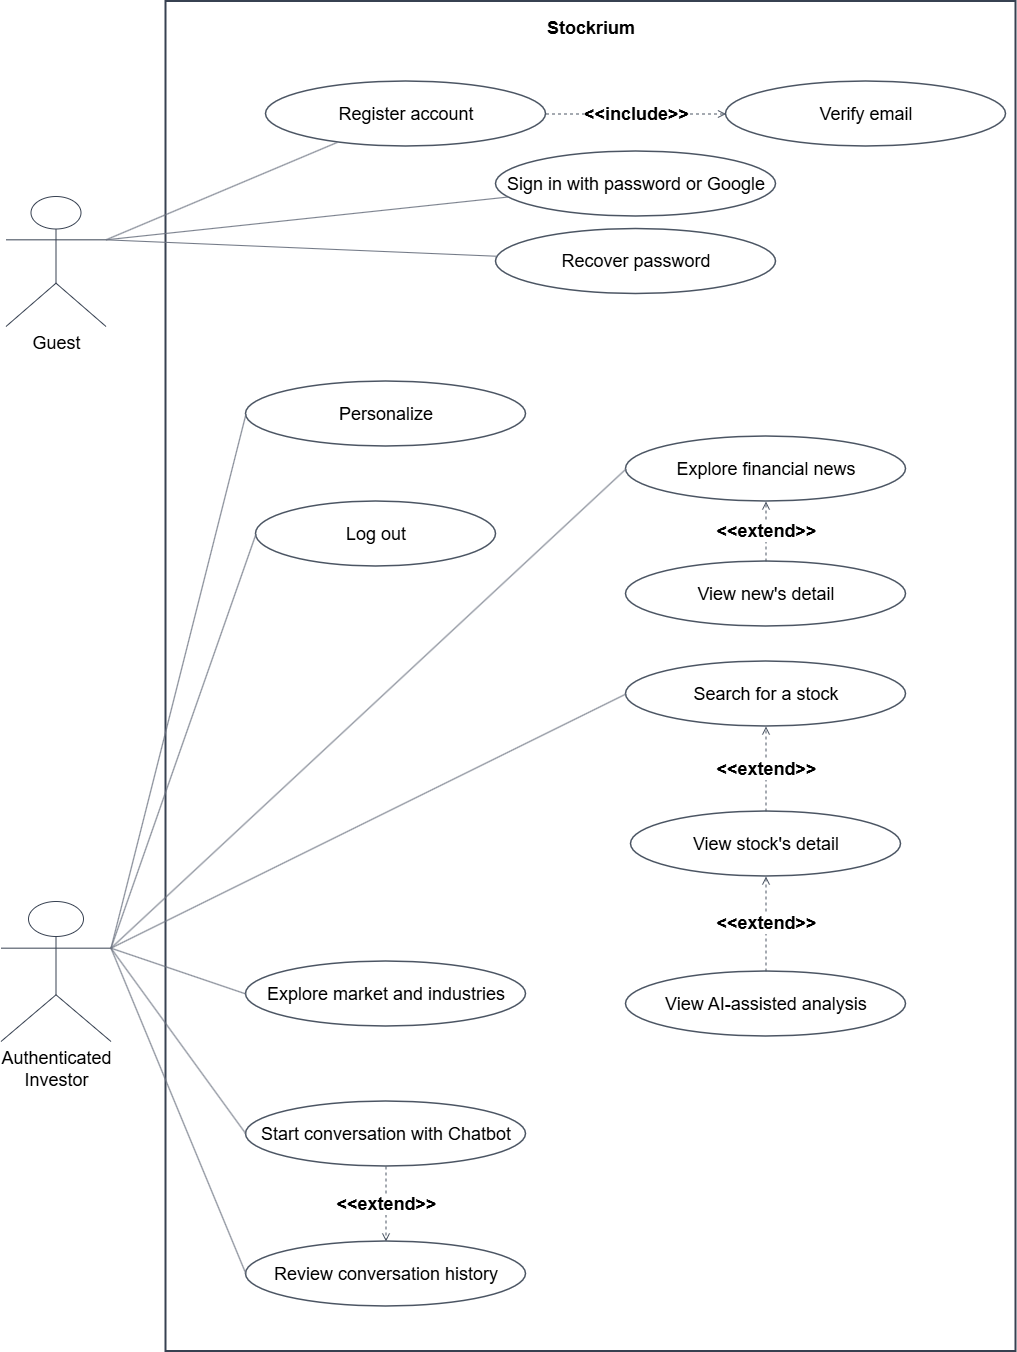
\includegraphics[width=\textwidth,height=0.8\textheight,keepaspectratio]{figures/chapter3/stockrium_use_case_model_stockrium.png}%
    }{%
        \fbox{\parbox[c][4.5cm][c]{0.92\textwidth}{\centering
        Missing figure:\\
        \texttt{figures/chapter3/stockrium\_use\_case\_model\_stockrium.png}}}%
    }
    \caption{Use-case model of the Stockrium mobile application}
    \label{fig:stockrium-mobile-use-case-model}
\end{figure}

\begin{figure}[H]
    \centering
    \IfFileExists{figures/chapter3/stockrium_use_case_model_web.png}{%
        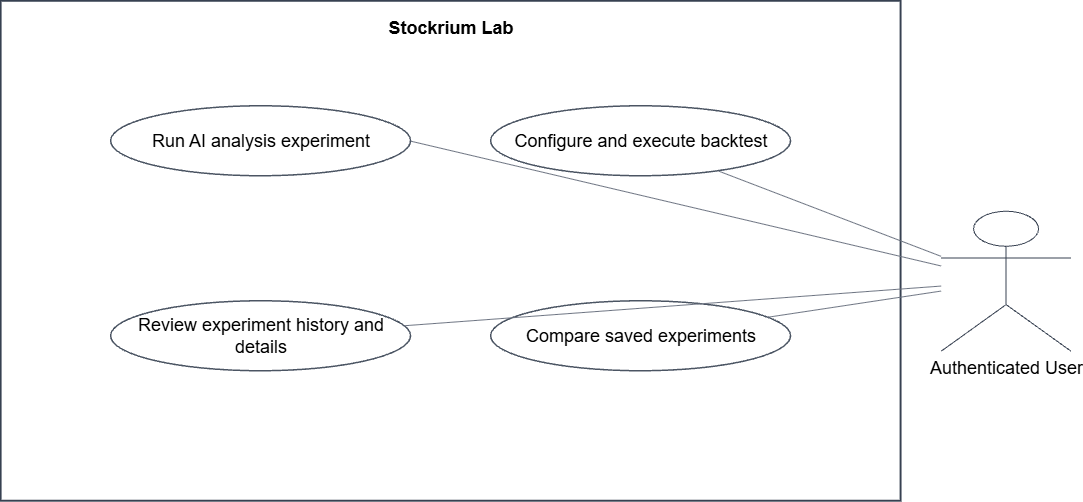
\includegraphics[width=\textwidth,height=0.8\textheight,keepaspectratio]{figures/chapter3/stockrium_use_case_model_web.png}%
    }{%
        \fbox{\parbox[c][4.5cm][c]{0.92\textwidth}{\centering
        Missing figure:\\
        \texttt{figures/chapter3/stockrium\_use\_case\_model\_web.png}}}%
    }
    \caption{Use-case model of Stockrium Lab}
    \label{fig:stockrium-web-use-case-model}
\end{figure}

{\small
\setlength\LTleft{\fill}
\setlength\LTright{\fill}
\begin{longtable}{>{\raggedright\arraybackslash}m{5.1cm} >{\raggedright\arraybackslash}m{8.7cm}}
    \caption{Use cases in the Stockrium mobile and experimentation interfaces}
    \label{tab:stockrium-use-cases} \\
    \toprule
    \textbf{Use case} & \textbf{Description} \\
    \midrule
    \endfirsthead
    \multicolumn{2}{l}{\small\itshape Table~\ref{tab:stockrium-use-cases} continued} \\
    \toprule
    \textbf{Use case} & \textbf{Description} \\
    \midrule
    \endhead
    \bottomrule
    \endfoot
    \multicolumn{2}{l}{\textbf{Mobile application}} \\
    Register account & Creates a new investor account and includes email verification. \\
    Verify email & Confirms ownership of the email address used to register the account. \\
    Sign in with password or Google & Authenticates the user through a supported sign-in method. \\
    Recover password & Restores access to an account with a forgotten password. \\
    Personalize & Adapts the application experience to the authenticated investor's preferences. \\
    Log out & Ends the current authenticated session. \\
    Explore financial news & Browses available financial articles. \\
    View news details & Opens the content and metadata of a selected financial article. \\
    Search for a stock & Finds a security by its symbol or company information. \\
    Explore market and industries & Reviews market conditions and industry groups. \\
    View stock details & Opens market, company, fundamental, technical, and news information for a selected stock. \\
    View AI-assisted analysis & Displays the AI-assisted assessment associated with the selected stock. \\
    Start conversation with Chatbot & Begins a conversational financial-support session. \\
    Review conversation history & Reopens previous chatbot sessions and messages. \\
    \midrule
    \multicolumn{2}{l}{\textbf{Stockrium Lab web workspace}} \\
    Run AI analysis experiment & Executes a supported analysis for one stock, VN30, or VN100 and stores the run as a user-owned experiment. \\
    Configure and execute backtest & Runs a supported historical simulation for one stock or VN30 and tracks its experiment status. \\
    Review experiment history and details & Filters previous experiments and opens their configuration, status, summary, detailed result, visualizations, and available reproducibility metadata. \\
    Compare saved experiments & Selects two to five experiments of the same type and compares their configurations and results side by side. \\
\end{longtable}
}

Market-data providers, news services, and language-model services are supporting dependencies rather than direct actors because they do not initiate the user goals shown in the model. Their interactions with Stockrium are described in the system architecture and data-pipeline sections of Chapter 4.

\subsection{Main Application Flows}
\label{subsec:main-application-flows}

The use cases form two primary experiences: an investor-facing mobile journey and the Stockrium Lab experimentation workflow. These flows describe user-visible behavior and intentionally treat the underlying multi-agent workflow as a single analytical service; its agents, state, and execution logic are presented in Chapter 4.

\subsubsection{Mobile Exploration and Stock-Analysis Flow}

A guest first completes onboarding and authenticates through registration, password sign-in, or the supported Google Sign-In flow. After authentication, the investor can enter a stock context from the market overview, search, financial news, or the watchlist. The stock-detail view consolidates price and volume charts, company information, fundamental data, technical indicators, and related news, allowing the investor to examine the available evidence before requesting an assessment.

The user may proceed with an automatic analysis configuration or manually select the evidence sources and their relative weights. The request combines the selected configuration, stock symbol, and saved investment horizon. Figure~\ref{fig:stockrium-primary-flow} summarizes the first part of the mobile journey, from account access and stock discovery to submission of the analysis request.

\begin{figure}[H]
    \centering
    \IfFileExists{figures/chapter3/mobile_decision_support_flow_part1.png}{%
        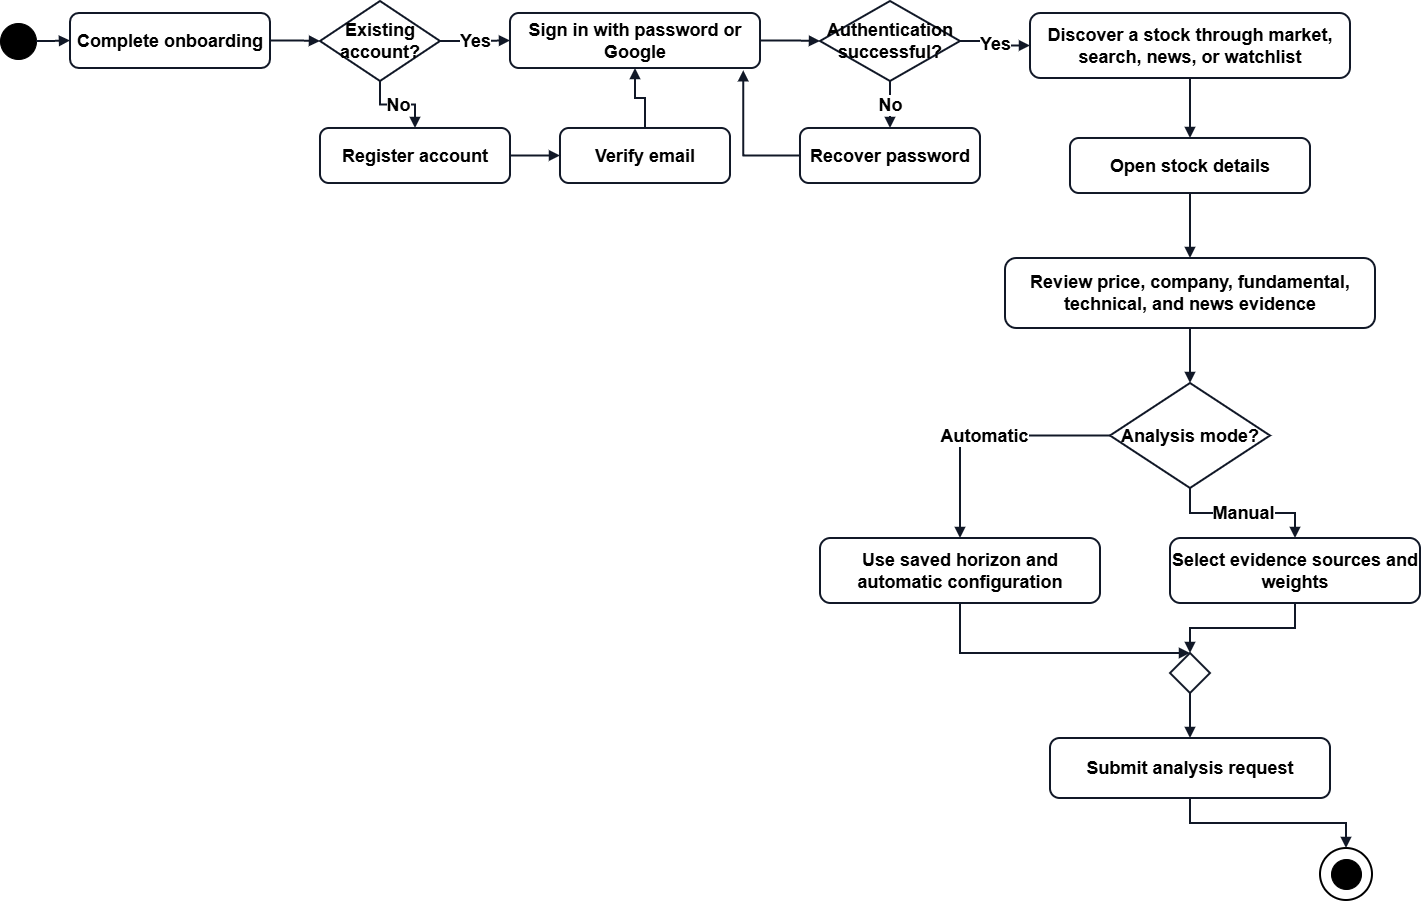
\includegraphics[width=\textwidth,height=\textheight,keepaspectratio]{figures/chapter3/mobile_decision_support_flow_part1.png}%
    }{%
        \fbox{\parbox[c][4.5cm][c]{0.92\textwidth}{\centering
        Export the Mermaid diagram as\\
        \texttt{figures/chapter3/mobile\_decision\_support\_flow\_part1.png}}}%
    }
    \caption{Mobile decision-support flow: account access, stock discovery, and analysis configuration}
    \label{fig:stockrium-primary-flow}
\end{figure}

After submission, Stockrium processes the enabled technical, fundamental, and news perspectives and returns either a \textit{Buy} or \textit{Wait} assessment. The result includes confidence and source-specific explanations; an accepted \textit{Buy} assessment may additionally contain an entry price, take-profit price, stop-loss price, and maximum holding period. Figure~\ref{fig:stockrium-analysis-result-flow} presents the second part of the journey, including evidence evaluation, recommendation validation, and subsequent user choices.

\begin{figure}[H]
    \centering
    \IfFileExists{figures/chapter3/mobile_decision_support_flow_part2.png}{%
        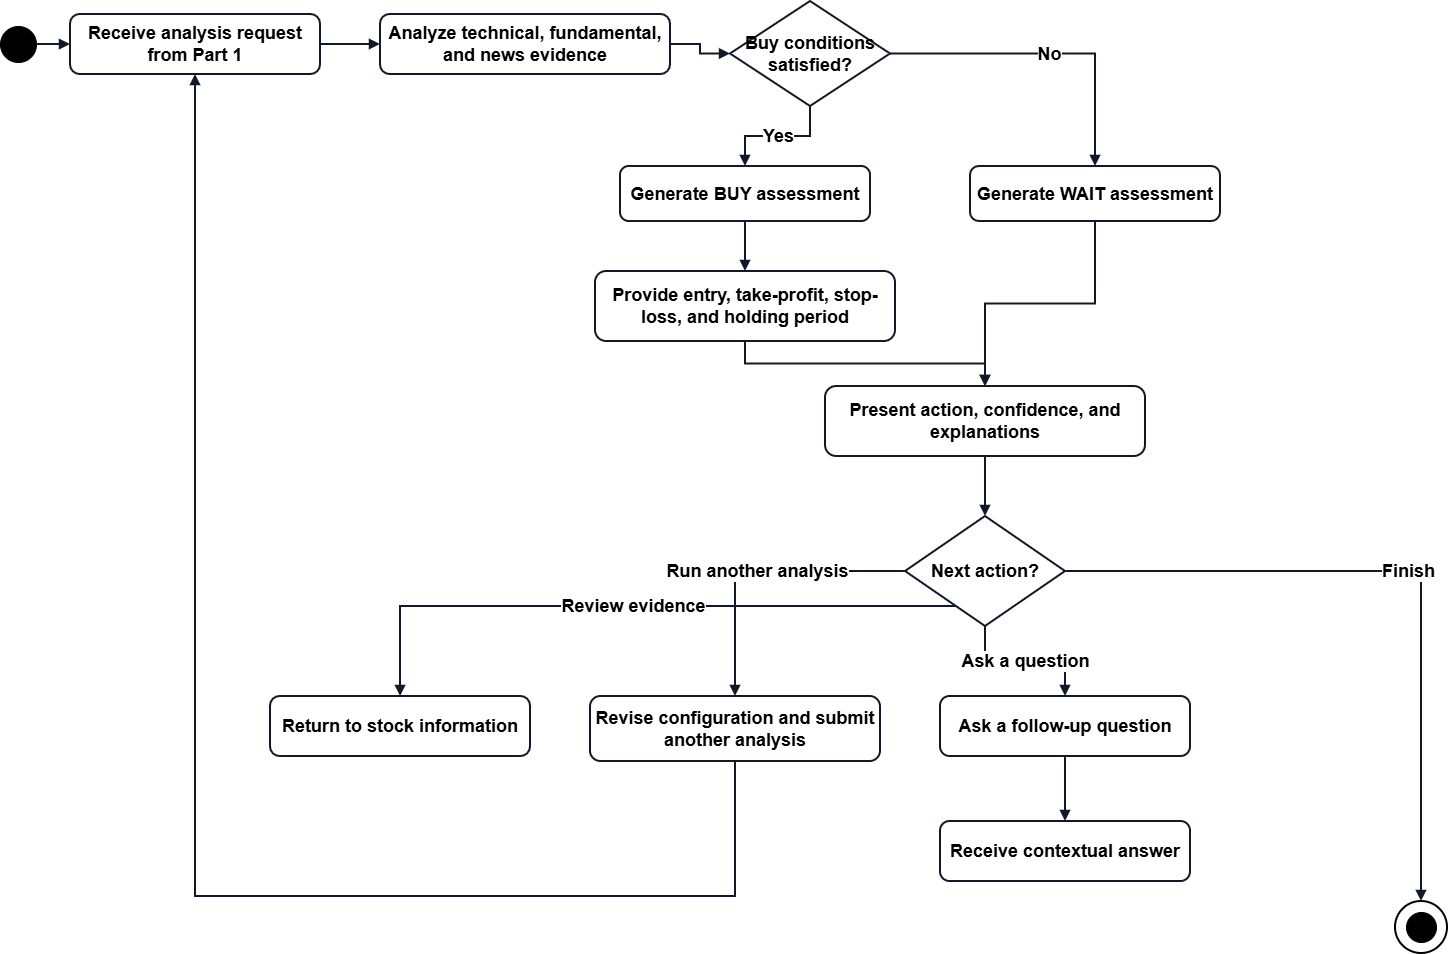
\includegraphics[width=\textwidth,height=\textheight,keepaspectratio]{figures/chapter3/mobile_decision_support_flow_part2.png}%
    }{%
        \fbox{\parbox[c][4.5cm][c]{0.92\textwidth}{\centering
        Export the Mermaid diagram as\\
        \texttt{figures/chapter3/mobile\_decision\_support\_flow\_part2.png}}}%
    }
    \caption{Mobile decision-support flow: analysis processing and recommendation}
    \label{fig:stockrium-analysis-result-flow}
\end{figure}

After reviewing the recommendation, the investor can return to the supporting charts and company data, revise the configuration, or update the watchlist. These paths form an iterative cycle in which the user continues to examine the evidence rather than acting solely on the generated action label.

\subsubsection{Stockrium Lab Experimentation and Comparison Flow}

An authenticated user opens Stockrium Lab to create a new experiment or revisit previous runs. AI-assisted analysis can be requested for an individual stock or the VN30 or VN100 universe. Backtesting can be executed for an individual stock or sequentially for the VN30 universe. The user names the experiment, selects the supported configuration, and submits it through the protected backend. Analysis results are returned after processing, whereas a backtest is accepted as a background job and can be monitored through its experiment status. Each run retains its configuration, summary, detailed output, and available reproducibility metadata under the current user's account.

The history view allows the user to filter experiments, reopen an analysis result, or load a completed backtest with its price chart, generated entries and exits, performance and risk measures, and comparison references. The user may also select from two to five experiments of the same type and compare their targets, inputs, pipeline metadata, and results side by side. This comparison is intended to expose configuration differences and pipeline behavior; a highlighted metric is not evidence that one experiment will remain superior in future market conditions. Figure~\ref{fig:stockrium-experimentation-flow} shows how execution, history review, and comparison return to the same Stockrium Lab workspace.

\begin{figure}[H]
    \centering
    \IfFileExists{figures/chapter3/experimentation_backtesting_flow.png}{%
        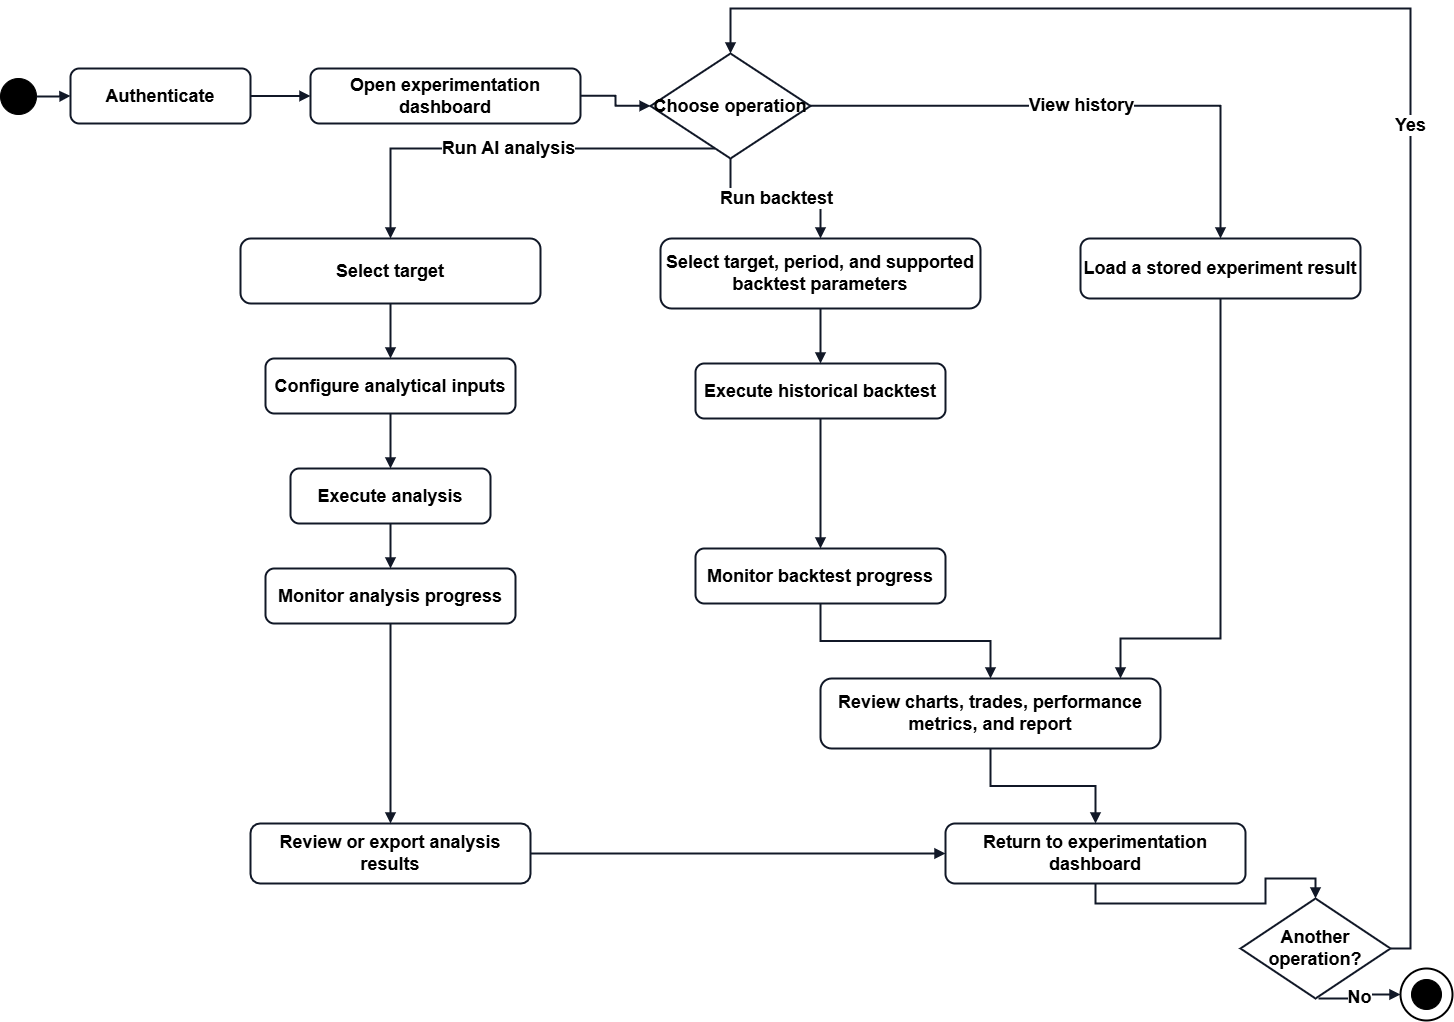
\includegraphics[width=\textwidth,height=\textheight,keepaspectratio]{figures/chapter3/experimentation_backtesting_flow.png}%
    }{%
        \fbox{\parbox[c][4.2cm][c]{0.92\textwidth}{\centering
        Export the Mermaid diagram as\\
        \texttt{figures/chapter3/experimentation\_backtesting\_flow.png}}}%
    }
    \caption{Stockrium Lab experimentation, history, and comparison flow}
    \label{fig:stockrium-experimentation-flow}
\end{figure}

The Stockrium Lab workflow supports controlled analysis, backtesting, history review, export, and experiment comparison. It is not a web trading platform and does not cause any real-market transaction. Together with the mobile journey, it positions Stockrium as an evidence-centered application and an inspectable environment in which users can test and compare the supported analytical pipeline without treating historical outcomes as guaranteed investment performance.

% ============================================================

% ============================================================
\section{Key Features}
\label{sec:key-features}

Stockrium provides a connected set of features for exploring the Vietnamese stock market, examining financial evidence, and obtaining AI-assisted analysis. The mobile application is intended for individual investors, while a separate administrative web interface supports controlled analysis and historical backtesting. This section summarizes the main user-visible capabilities; their architecture and implementation are presented in Chapter 4.

\subsection{Authentication and Account Management}
\label{subsec:authentication-account-management}

Users can create an account with an email address, verify it through a one-time password, and sign in using either a password or Google Sign-In. The application also supports password recovery, session persistence, and secure sign-out. After authentication, users can manage their investment horizon, conversation history, theme, and language preferences. They can also add or remove stocks from a personal watchlist for later monitoring. This watchlist stores only selected symbols and does not manage quantities, purchase prices, profit and loss, or capital allocation. The security mechanisms used to protect credentials and sessions are discussed in Chapter 4.

\subsection{Market Overview and Stock Discovery}
\label{subsec:market-overview-discovery}

The Overview and Market tabs provide a concise view of current Vietnamese market conditions. Users can inspect major indices, industry movements, financial news, and stock collections such as top gainers, top decliners, highly traded stocks, and frequently followed symbols. The search function allows users to locate listed companies by stock symbol or company name and revisit previous queries through their search history. These discovery features support navigation rather than constitute investment recommendations. A selected index, industry, stock, or article can be opened for further examination.

\subsection{Stock Details and Interactive Technical Charts}
\label{subsec:stock-details-charts}

The stock-detail screen combines current and historical market data with company information, fundamental indicators, related news, and similar securities. Interactive area and candlestick charts allow users to examine price, volume, and selected technical indicators over different periods. The same screen also presents the company's business profile, leadership information, historical financial performance, financial statements, and representative measures of valuation, profitability, liquidity, and financial strength. Together, these features help users compare market behavior with the company's operating condition. The displayed information supports independent inspection but does not place orders or initiate financial transactions; AI-assisted analysis is requested separately.

\subsection{Financial News Exploration}
\label{subsec:financial-news-exploration}

The News tab organizes financial articles into business, macroeconomic, and topic-based views. Stock-specific articles are also accessible from the corresponding stock-detail screen, allowing users to relate company events and market sentiment to price and fundamental data. The collection pipeline enriches stored articles with short summaries and positive, neutral, or negative sentiment labels. The mobile application presents article content and surfaces sentiment in selected news views, while the processed fields also provide evidence for subsequent analysis. News collection and processing occur in a separate scheduled pipeline described in Chapter 4.

\subsection{Investment-Horizon Profile}
\label{subsec:investment-horizon-profile}

Users can save an intended investment horizon as short term (under three months), medium term (three to twelve months), or long term (over one year). When an AI analysis is requested, the system maps this preference to a daily, weekly, or monthly technical-analysis interval. For an accepted \textit{Buy} assessment, the horizon also determines the permitted ranges for take-profit, stop-loss, and maximum holding period. Within the current application scope, this profile considers only investment horizon and is not a comprehensive assessment of financial capacity or psychological risk tolerance.

\subsection{Configurable AI Analysis}
\label{subsec:configurable-ai-analysis}

Stockrium provides automatic and manual modes for AI-assisted stock analysis. Automatic mode uses all available analytical perspectives with default weights determined by the saved investment horizon. Manual mode allows the user to enable or disable news, individual technical indicators, and fundamental-indicator categories, and to adjust the relative weights of the technical, fundamental, and news perspectives. The multi-agent system coordinates the enabled components and returns a \textit{Buy} or \textit{Wait} assessment with a normalized confidence score, technical, fundamental, and news scores, and written explanations. Confidence represents the system's internal strength of evidence and is not a probability of future profit. A \textit{Buy} result may also include a proposed entry price, take-profit price, stop-loss price, and maximum holding period consistent with the selected horizon. The feature provides a simple default path for beginners and greater control for experienced users, while its outputs remain decision-support information rather than guaranteed returns or executable orders.

\subsection{Conversational Financial Assistant}
\label{subsec:conversational-financial-assistant}

The conversational assistant allows users to ask natural-language questions about the financial and market information available in Stockrium. Conversations are stored as sessions so that users can create, reopen, continue, or delete previous discussions. A conversation may begin as a general inquiry or from an AI-analysis result, enabling follow-up questions about the recommendation and its supporting evidence. The assistant explains and summarizes available information but does not act as a brokerage service or licensed financial adviser.

\subsection{Administrative Analysis and Backtesting}
\label{subsec:administrative-analysis-backtesting}

The administrative web interface provides protected tools for running stock analysis and historical backtests. An administrator can request AI-assisted analysis for an individual stock or the VN30 or VN100 index basket. Backtesting can be configured for an individual stock or executed sequentially across VN30 using the supported inputs and analytical selections. The administrator can monitor batch progress and inspect or export the resulting reports. Backtesting summarizes historical behavior through measures such as total return, win rate, Sharpe ratio, maximum drawdown, and trade history, with visualizations linking generated signals to price data. This interface is an internal evaluation and operational tool; it is not publicly deployed and does not execute live securities transactions.

Together, these features form a decision-support environment that connects market discovery, evidence inspection, AI-assisted synthesis, explanation, and conversational follow-up. Stockrium helps users organize and interpret Vietnamese market information while keeping investment decisions and any subsequent transactions under the user's responsibility.

% ============================================================

\clearpage
\chapter{System Design and Implementation}

\textit{This chapter describes the architecture and implementation of Stockrium. It explains how the mobile client, administrative dashboard, backend services, persistent data stores, external data pipelines, agentic analysis workflow, conversational assistant, backtesting framework, security mechanisms, and deployment environment cooperate to realize the proposed application.}

% ============================================================
\section{System Architecture Overview}
\label{sec:system-architecture-overview}

Stockrium follows a client--server architecture supported by independent background and offline data-acquisition pipelines. The React Native mobile application is the primary interface for individual investors, while an internal experimentation and backtesting web interface allows authorized evaluators to run controlled analysis and historical experiments. Both clients communicate with a FastAPI backend that centralizes authentication, business logic, data access, agentic AI and conversational workflows, and standardized API responses.

Supabase PostgreSQL stores the application's durable business, market, financial, news, and conversational data, while Redis maintains temporary authentication and verification state. Separate workers collect and prepare information from external sources such as SSI and online news providers. This separation keeps provider credentials and processing logic outside the clients and allows most user requests to read normalized data that have already been prepared.

\subsection{Architectural Requirements}
\label{subsec:architectural-requirements}

The architecture must support mobile market exploration, configurable agentic AI analysis, conversational queries, and controlled backtesting without coupling these responsibilities to the user interface. It must integrate heterogeneous financial evidence, protect user-specific and restricted experimentation operations, preserve conversation state, and update market and news data without blocking normal requests. Maintainability is supported by separating presentation, domain services, agentic AI and conversational workflows, and data access. Most importantly, the architecture reflects the application's decision-support scope: no component connects to a brokerage account, transfers funds, or executes securities transactions.

Several quality attributes influence this organization. Security requires provider keys and privileged data access to remain on the server side. Responsiveness requires ordinary mobile requests to read prepared records instead of waiting for crawlers or large imports. Maintainability requires the API, analytical workflows, and acquisition jobs to evolve independently, while traceability is supported by structured results and persistent records for conversations and historical experiments. The architecture therefore prioritizes clear responsibility boundaries, traceable processing, and repeatable evaluation rather than the low-latency execution required by a trading platform.

\subsection{Logical Architecture}
\label{subsec:logical-architecture}

The logical architecture is organized into presentation, API and application services, AI and evaluation, data integration, and persistence. Background workers connect external providers to the data layer independently of user requests. Figure~\ref{fig:stockrium-overall-architecture} summarizes the principal components and their relationships.

\begin{figure}[H]
    \centering
    \IfFileExists{figures/chapter4/stockrium_client_server_architecture.png}{%
        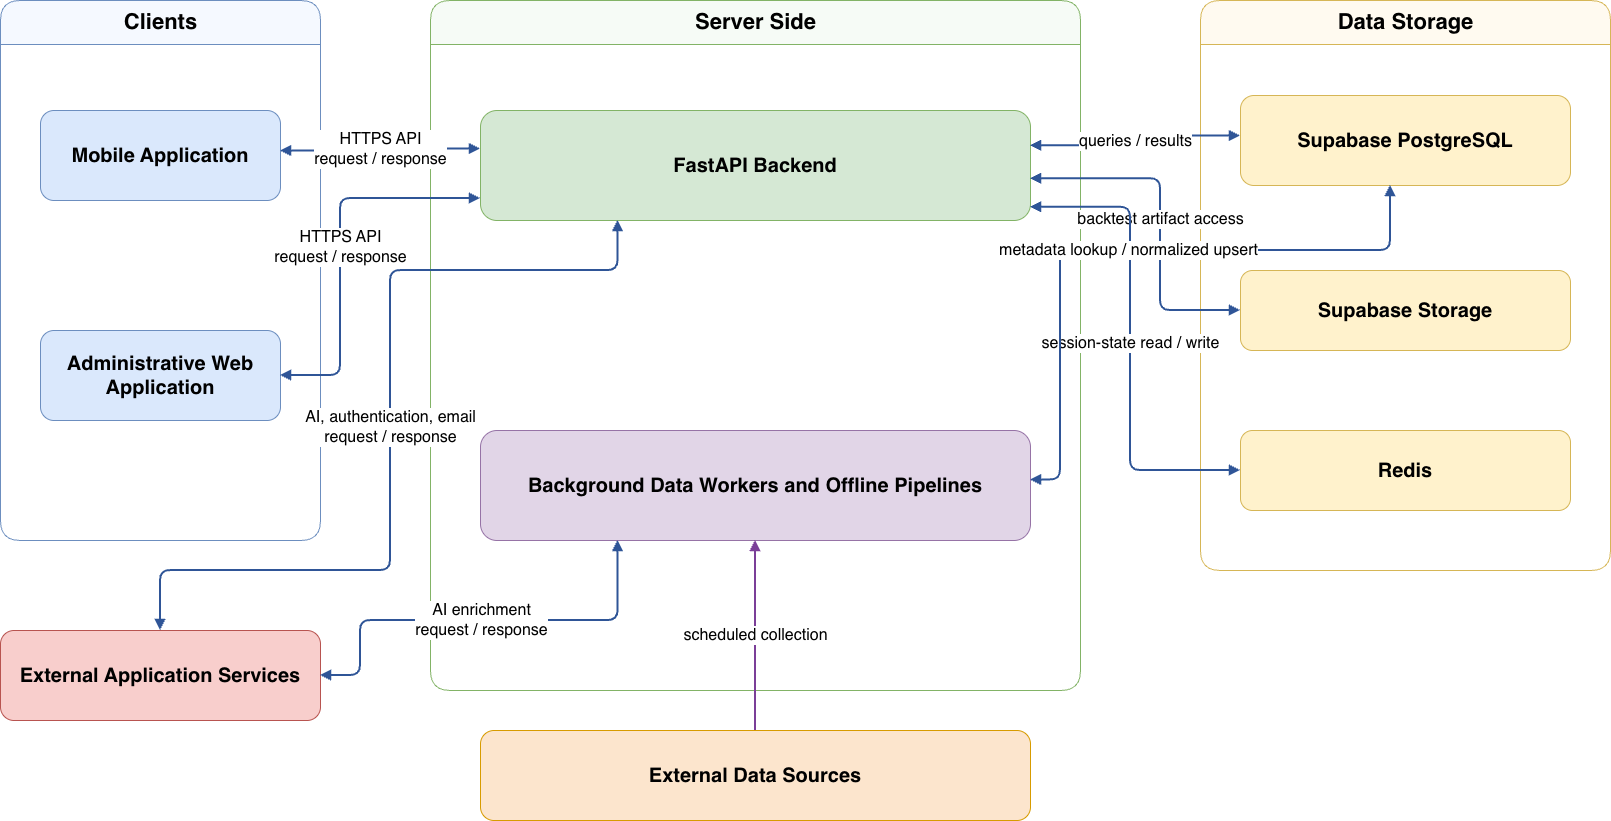
\includegraphics[width=\textwidth,height=0.78\textheight,keepaspectratio]{figures/chapter4/stockrium_client_server_architecture.png}%
    }{%
        \fbox{\parbox[c][5.5cm][c]{0.92\textwidth}{\centering
        Export the Draw.io diagram as\\
        \texttt{figures/chapter4/stockrium\_client\_server\_architecture.png}}}%
    }
    \caption{Overall logical architecture of Stockrium}
    \label{fig:stockrium-overall-architecture}
\end{figure}

On the client side, the mobile application and experimentation web interface serve different actors while sharing the same server boundary. The mobile application supports everyday investor activities, including authentication, market discovery, stock details, charts, news, the watchlist, investment-horizon management, AI-assisted analysis, and conversational follow-up. It retains only interface state, user preferences, and securely stored authentication tokens; authoritative financial and user data remain on the server. The experimentation interface is restricted to authorized evaluators. It supports AI-assisted analysis for an individual stock, VN30, or VN100 and backtesting for an individual stock or VN30, together with progress monitoring, result inspection, and export. Backtesting evaluates Stockrium's analytical pipeline and supported configurations; it is not a general-purpose strategy builder or a publicly deployed web equivalent of the mobile product.

On the server side, FastAPI acts as the single entry point for Stockrium application requests from both clients. It validates request schemas, authenticates the current session, checks elevated-role authorization where required, invokes the relevant application service, and returns the standardized Stockrium response structure. Domain services organize operations for accounts, market data, company profiles, financial statements, articles, watchlists, search history, and investment horizons. This route--service separation prevents the clients from depending on database-specific queries and permits the same business operations to be reused by analytical workflow components, chatbot tools, or backtesting services.

The server also owns the computation-intensive and security-sensitive capabilities. The stock-analysis workflow coordinates technical, fundamental, and news evidence before producing a structured recommendation. The conversational workflow maintains multi-turn state and selects suitable financial tools, while the backtesting subsystem applies the analytical logic to historical data under supported backtest inputs. These components may call external language-model services, but API keys, prompts, validation rules, and post-processing remain within the server-side environment. Their internal designs are described separately later in this chapter.

The storage side is divided according to data lifetime and format. Supabase PostgreSQL is the authoritative relational store for accounts, personalization, stocks, prices, market indices, company records, financial statements, articles, classifications, chat-session metadata, and LangGraph checkpoints. Supabase Storage holds backtest artifacts that are more suitable as files than relational rows. Redis stores revocable or short-lived authentication state, including access and refresh token registrations, one-time passwords, attempt counters, and password-reset sessions. Interactive client operations retrieve and update these stores through the FastAPI backend, while authorized acquisition workers access the required data stores independently of client requests.

Background workers form a second server-side execution path that is independent of interactive API requests. The market-price worker receives SSI data, prepares intraday and daily records, and performs post-session normalization. The article worker discovers and extracts financial news, checks duplicates, generates summaries and sentiment labels, links articles to stocks or categories, and persists the processed results. Company and fundamental utilities collect profile and financial information through Selenium and downloadable files before transforming it with pandas. These jobs can read database metadata or existing records before upserting normalized results into PostgreSQL.

External application services support both synchronous and background operations. OpenAI models are used by the analytical workflows and selected enrichment jobs, while Resend delivers account-verification email. These services are accessed by the backend or workers so that credentials and output validation remain in the server-side environment. Google Sign-In follows a different boundary: the mobile application initiates authentication with Google Identity, receives an identity token, and sends it to the backend for verification and issuance of Stockrium access and refresh tokens. None of these request--response integrations is an authoritative source of Stockrium's business or market records.

\subsection{End-to-End Request Flows}
\label{subsec:end-to-end-request-flows}

For an ordinary data-retrieval request, a client sends a Hypertext Transfer Protocol (HTTP) request to FastAPI and includes a Stockrium authentication token where required; deployed mobile requests use Hypertext Transfer Protocol Secure (HTTPS). The route validates the input and resolves the current user before invoking a domain service. The service reads the corresponding prepared records from PostgreSQL, applies any required transformation, and returns them through the standard response envelope. The client then maps the response into cards, lists, charts, or detail views. User actions such as updating the watchlist, search history, or investment horizon follow the same path but write the authorized change before returning the updated state.

An AI-analysis request follows the same client--server boundary but invokes a server-side graph after the relevant market, fundamental, and news evidence has been retrieved. Only the selected analytical components participate, and their outputs are synthesized and validated before the result is returned to the client. A conversational request additionally loads and updates its LangGraph checkpoint, whereas a controlled backtest repeatedly applies analytical logic to historical records and may expose or store an experiment artifact. Although these operations differ in duration and state, none bypasses backend authentication or grants a client direct access to the database or model provider.

Data acquisition follows a path independent of interactive requests. At scheduled times, during market hours, or through a controlled offline preparation run, a worker or utility reads from its external provider, normalizes the received representation, checks required database context, and upserts the prepared data into PostgreSQL. The FastAPI service later reads the resulting records in response to client requests. Separating this path from the web-server lifecycle prevents a market stream, browser crawler, article-processing batch, or large import from delaying ordinary API traffic and avoids duplicating scheduled jobs when the API process restarts or scales.

Overall, Stockrium combines thin client applications, a validated FastAPI boundary, modular domain and AI services, independent acquisition pipelines, and storage selected according to data lifetime. The following sections describe each of these areas in greater detail.

% ============================================================

% ============================================================
\section{Mobile Application Architecture}
\label{sec:mobile-application-architecture}

The Stockrium mobile application is implemented with React Native, Expo, TypeScript, and Expo Router. Its architecture follows a layered, screen-oriented structure in which every route represents a user-visible task and reusable components encapsulate market cards, charts, forms, bottom sheets, and financial sections. The client is intentionally responsible for interaction, presentation, lightweight input validation, and local preferences. Authentication decisions, authoritative financial data, technical calculations, and AI execution remain behind the backend API.

The application combines Expo Router's file-based stack navigation with a custom five-tab interface. File-based routes manage transitions between major screens, while the main application shell uses a pager to support horizontal tab movement and preserve the distinctive central Chatbot control. This hybrid navigation model provides conventional stack behavior for detailed tasks without restricting the visual and interaction design of the primary tabs.

\subsection{Layered Mobile Architecture}
\label{subsec:layered-mobile-architecture}

Figure~\ref{fig:stockrium-mobile-architecture} presents the mobile client as a layered architecture. The layers separate application-wide composition, user-facing presentation, state ownership, API access, and persistent device storage. The arrows represent the principal dependencies and data exchanges rather than a strict invocation sequence.

\begin{figure}[H]
    \centering
    \IfFileExists{figures/chapter4/stockrium_mobile_architecture.png}{%
        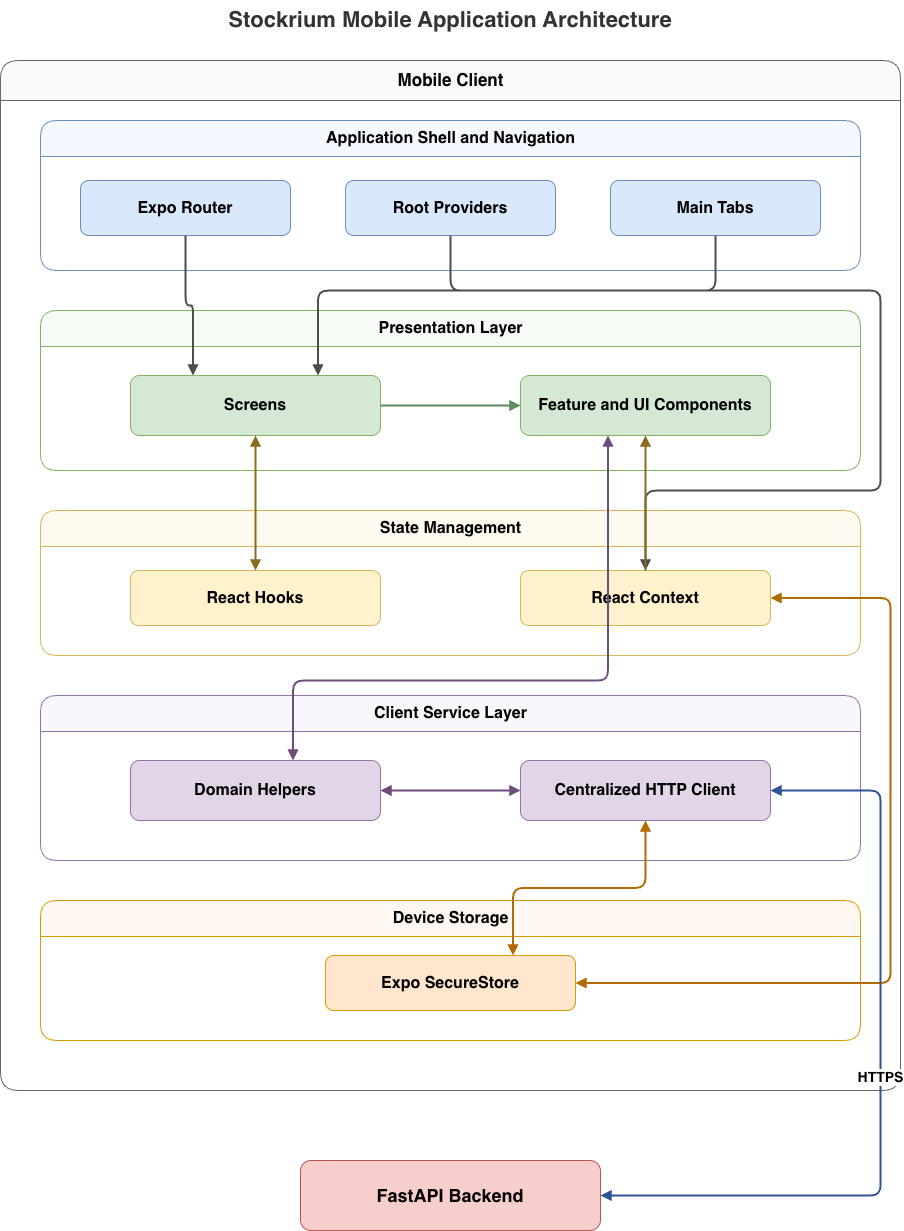
\includegraphics[width=0.72\textwidth,height=0.82\textheight,keepaspectratio]{figures/chapter4/stockrium_mobile_architecture.png}%
    }{%
        \fbox{\parbox[c][6.0cm][c]{0.88\textwidth}{\centering
        Expected architecture diagram:\\
        \texttt{figures/chapter4/stockrium\_mobile\_architecture.png}}}%
    }
    \caption{Layered architecture of the Stockrium mobile application}
    \label{fig:stockrium-mobile-architecture}
\end{figure}

The application shell and navigation layer establishes the client-wide execution environment. Expo Router maps files to stack destinations, the root providers supply safe-area, gesture, localization, and theme facilities, and the custom main tabs coordinate the five primary application areas. This layer determines which screen is active and ensures that shared infrastructure is available before feature content is rendered.

The presentation layer contains route-level screens and reusable feature and UI components. Screens coordinate a user task, receive route parameters, and compose the required feature components. Reusable components encapsulate domain-specific sections and common interface elements so that market data, stock details, authentication controls, news content, and analysis results can be presented consistently without duplicating implementation across routes.

State is kept close to the scope in which it is needed. React Hooks manage transient screen or component state, including loading indicators, selections, form values, and fetched results. React Context distributes the smaller set of cross-cutting presentation preferences, particularly theme and language. Values that must survive application restarts, such as session tokens and selected local preferences, are stored through Expo SecureStore instead of remaining only in memory.

The client service layer separates UI code from transport details. Feature-oriented domain helpers translate screen operations into typed application requests and delegate them to the centralized HTTP client. The HTTP client constructs HTTPS requests to the FastAPI backend, attaches stored credentials, coordinates token refresh, and returns parsed responses to the calling helper. It also exchanges session data with SecureStore, while providers restore persisted preferences into React Context. This separation allows screens and components to focus on interaction and presentation, while authentication recovery, endpoint construction, and secure persistence remain centralized.

\subsection{Navigation Structure}
\label{subsec:mobile-navigation-structure}

The root layout establishes the providers and infrastructure that every screen requires. It first loads the Roboto font family and then nests the application inside a safe-area provider, gesture-handler root, localization provider, and theme provider. An Expo Router stack manages screen transitions with the default header disabled because Stockrium screens provide their own headers. A global session-expired modal is rendered beside the stack so that authentication failure can be communicated regardless of which screen is currently active.

The index route acts as a navigation gateway rather than a visible home screen. It reads the persistent onboarding flag and the stored session. If onboarding has not been completed, the user is redirected to the Onboarding route. If onboarding is complete, both token values are present, and the refresh token has not expired, the user is redirected to the main Tabs route. Otherwise, the Authentication route is opened. The gateway does not require the access token itself to remain valid because an expired access token can be renewed transparently by the centralized HTTP client.

The authentication branch contains two related paths. The account-creation path proceeds from the sign-up form to one-time password (OTP) verification. Successful verification confirms the email address and returns the user to authentication; it does not create an authenticated session automatically. The account-recovery path proceeds from email input to OTP verification and then to the new-password screen before returning to authentication. Returning users can sign in with application credentials or Google and move directly to the Tabs route. Navigation replacement is used after onboarding or successful authentication so that the Android back action does not return the user to a completed entry screen.

The main shell contains Overview, Market, Chatbot, News, and Profile. It is implemented with a pager and a custom bottom bar rather than Expo Router's default tab navigator. A tab is mounted only after it has been visited, reducing the initial work required to construct data-heavy market and news screens. The active-tab indicator is animated, and the Chatbot is represented by a raised central button instead of a conventional tab item. Swiping the pager or selecting a bottom-bar item updates the same active index.

Figure~\ref{fig:mobile-navigation-structure} summarizes the principal route relationships. It groups routes according to user goals rather than listing every modal bottom sheet as an independent destination.

\begin{figure}[H]
    \centering
    \IfFileExists{figures/chapter4/stockrium_mobile_navigation_structure.png}{%
        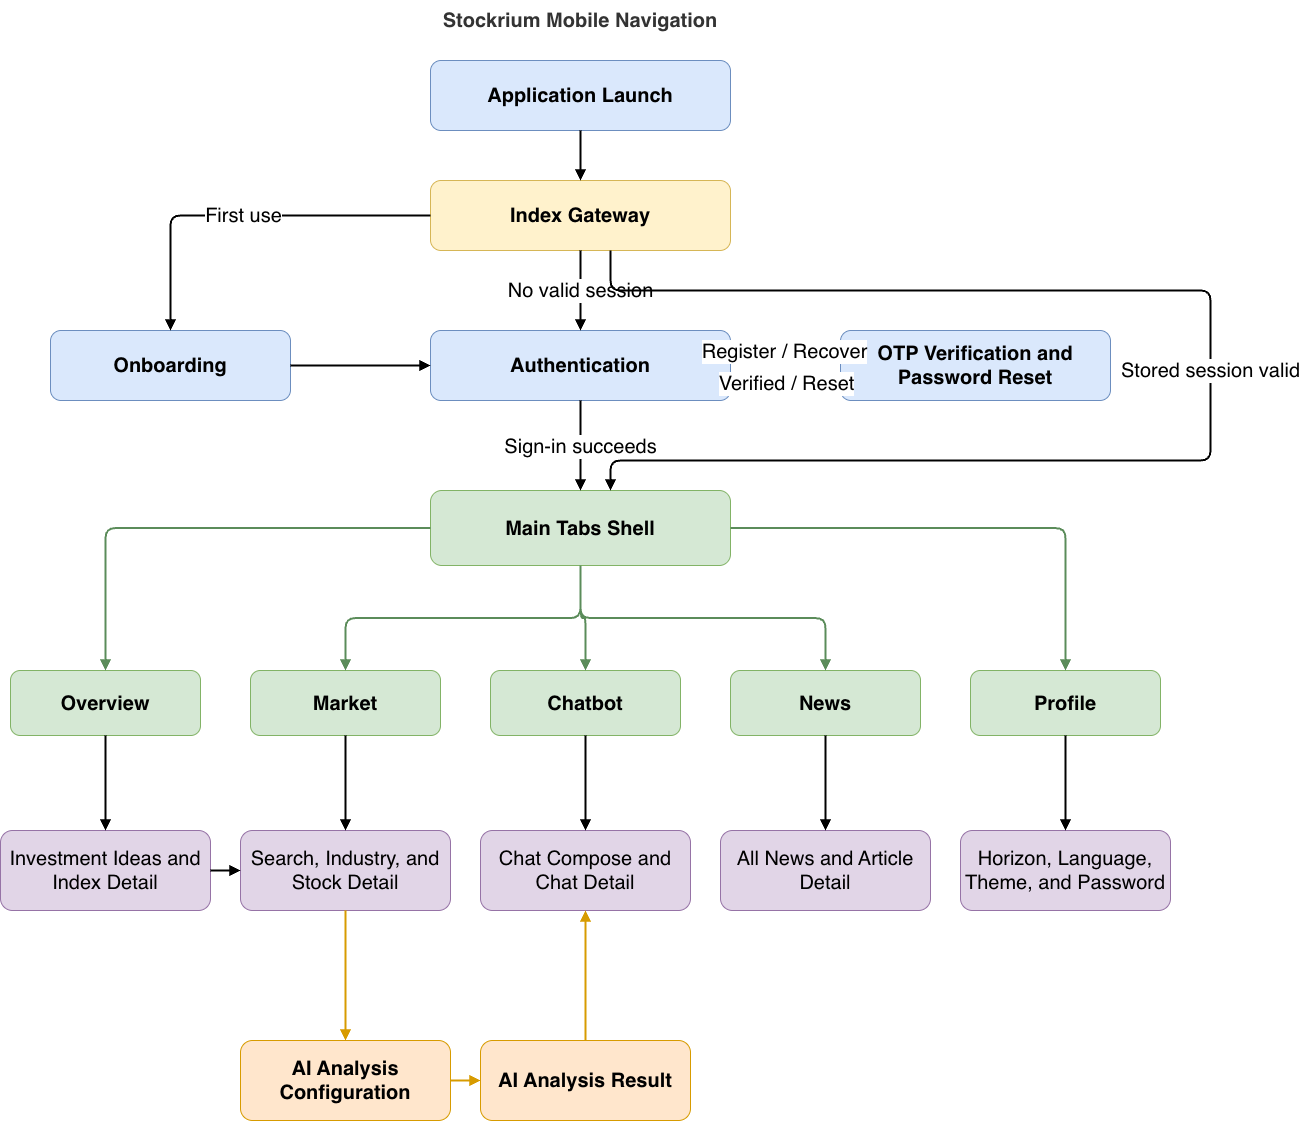
\includegraphics[width=0.96\textwidth,height=0.82\textheight,keepaspectratio]{figures/chapter4/stockrium_mobile_navigation_structure.png}%
    }{%
        \fbox{\parbox[c][5.5cm][c]{0.92\textwidth}{\centering
        Export the Draw.io diagram as\\
        \texttt{figures/chapter4/stockrium\_mobile\_navigation\_structure.png}}}%
    }
    \caption{Principal navigation structure of the Stockrium mobile application}
    \label{fig:mobile-navigation-structure}
\end{figure}

The Stock Detail route is a particularly important navigation hub. It can be opened from search results, watchlist entries, investment-idea lists, industry visualizations, market highlights, and related-stock cards. It receives the stock symbol as a route parameter and passes the same symbol to its child sections. A floating AI button opens the configuration route with that symbol, after which the result route receives the analysis mode and serialized manual selection. This parameterized navigation keeps the user focused on one company across data inspection and AI analysis.

News and chatbot routes follow a similar pattern. General or categorized lists open a shared article-detail route using article parameters. The Chatbot tab displays available sessions; composing or selecting a session opens Chat Detail with a session identifier. An AI result can create and seed a new session before navigating to that same Chat Detail route, allowing ordinary conversations and analysis follow-ups to reuse one interface.

\subsection{API Integration and Client State}
\label{subsec:api-integration-client-state}

The mobile application does not call \texttt{fetch} directly from every screen. Feature-specific helpers expose typed functions such as market-index retrieval, stock-price retrieval, company-profile retrieval, watchlist operations, investment-horizon persistence, analysis execution, and chat-session management. These helpers build endpoint paths and request bodies, then delegate network behavior to a single HTTP function. This structure keeps route strings, response interpretation, and authentication recovery out of visual components.

\subsubsection{Base URL and Request Construction}

The API base URL depends on the build environment. Production builds use the deployed Railway backend. During development, iOS uses the local host, Android or a physical Expo device derives the development machine address from the Metro host when possible, and the Android-emulator fallback uses its host mapping. Centralizing this decision prevents screens from embedding environment-specific addresses.

For each request, the shared client reads the access and refresh tokens from SecureStore. It constructs JSON headers and adds the bearer access token when present. The feature helper then receives the parsed Stockrium response and converts its error code and data into a compact success/failure shape appropriate for the calling screen.

\subsubsection{Automatic Token Refresh}

An HTTP 401 Unauthorized response triggers coordinated token renewal. If no refresh is currently running, the failed request becomes the refresh leader and submits the stored refresh token to the authentication endpoint. Other requests that receive 401 during this interval subscribe to the same operation instead of issuing additional refresh calls. If renewal succeeds, a new access token is saved and the subscribed requests retry using the new value, followed by the original leader request. Figure~\ref{fig:mobile-token-refresh-flow} illustrates this sequence.

\begin{figure}[H]
    \centering
    \resizebox{0.86\textwidth}{!}{%
    \begin{tikzpicture}[
        box/.style={draw, rounded corners=5pt, fill=blue!7, minimum width=3.0cm, minimum height=1.0cm, align=center, font=\small},
        decision/.style={draw, rounded corners=10pt, fill=yellow!15, minimum width=2.8cm, minimum height=1.0cm, align=center, font=\small},
        action/.style={draw, rounded corners=5pt, fill=green!9, minimum width=3.2cm, minimum height=1.0cm, align=center, font=\small},
        failure/.style={draw, rounded corners=5pt, fill=red!8, minimum width=3.2cm, minimum height=1.0cm, align=center, font=\small},
        flow/.style={-{Latex[length=2.2mm]}, line width=0.65pt, gray!80},
        guard/.style={font=\scriptsize, text=black}
    ]
        \node[box] (screen) at (0,0) {Screen calls a\\feature helper};
        \node[box] (session) at (0,-1.8) {Read session and\\send bearer request};
        \node[decision] (status) at (0,-3.6) {Response\\status};
        \node[action] (success) at (5.0,-3.6) {Return parsed response\\to the screen};
        \node[decision] (active) at (0,-5.5) {Refresh already\\in progress?};
        \node[action] (wait) at (-3.7,-7.5) {Subscribe and wait for\\the shared new token};
        \node[action] (refresh) at (3.7,-7.5) {Call refresh endpoint\\with refresh token};
        \node[decision] (refreshstatus) at (3.7,-9.4) {Refresh\\succeeds?};
        \node[action] (retry) at (0,-11.4) {Save token, notify\\subscribers, and retry};
        \node[failure] (expired) at (7.4,-11.4) {Emit session-expired\\event and show modal};

        \draw[flow] (screen.south) -- (session.north);
        \draw[flow] (session.south) -- (status.north);
        \draw[flow] (status.east) -- node[above, guard] {not 401} (success.west);
        \draw[flow] (status.south) -- node[right, guard] {401} (active.north);
        \draw[flow] (active.south west) -- node[above left, guard] {yes} (wait.north east);
        \draw[flow] (active.south east) -- node[above right, guard] {no} (refresh.north west);
        \draw[flow] (refresh.south) -- (refreshstatus.north);
        \draw[flow] (refreshstatus.south west) -- node[above left, guard] {yes} (retry.north east);
        \draw[flow] (refreshstatus.south east) -- node[above right, guard] {no} (expired.north west);
        \draw[flow] (wait.south) |- node[left, guard] {on success} (retry.west);
    \end{tikzpicture}%
    }
    \caption{Coordinated access-token refresh in the mobile HTTP client}
    \label{fig:mobile-token-refresh-flow}
\end{figure}

If refresh fails or returns incomplete token data, the client emits a global authentication-expired event. The modal registered in the root layout becomes visible, removes local session data after confirmation, and replaces the current route with Authentication. This event-based mechanism avoids passing an expiration callback through every component.

\subsubsection{State Scope and Persistence}

Stockrium uses local React state for screen-specific data, React context for a small number of application-wide preferences, SecureStore for persistent device state, and backend storage for user-owned domain state. A large global state framework is not required because market and detail screens can request their own independent data and because user-specific records such as watchlist entries and conversations already have authoritative server representations.

\begin{table}[H]
    \centering
    \caption{Client-state scopes in the Stockrium mobile application}
    \label{tab:client-state-scopes}
    \small
    \begin{tabularx}{\textwidth}{>{\raggedright\arraybackslash}p{3.1cm} >{\raggedright\arraybackslash}p{4.1cm} X}
        \toprule
        \textbf{State scope} & \textbf{Mechanism} & \textbf{Examples} \\
        \midrule
        Screen-local transient state & React state, refs, memoization, effects, and a keyboard-visibility hook & Loading flags, fetched lists, chart type, selected time frame, active indicator, keyboard visibility, bottom-sheet visibility, search text, selected radar axis, and form validation. \\
        \addlinespace
        Cross-screen presentation state & React Context & Current light/dark theme, selected language, and translated text lookup. \\
        \addlinespace
        Persistent device state & Expo SecureStore & Access token, refresh token, onboarding completion, theme, language, and the saved AI-analysis preset. \\
        \addlinespace
        Navigation state & Expo Router and the custom PagerView & Current stack route, route parameters, active main tab, and the set of tabs that have been visited and mounted. \\
        \addlinespace
        Global transient events & Event emitters & Authentication expiration and programmatic switching of the custom tab shell. \\
        \addlinespace
        Authoritative user data & Backend API and Supabase & Watchlist symbols, search history, investment horizon, account profile, chat sessions, and chat messages. \\
        \bottomrule
    \end{tabularx}
\end{table}

The Theme and Localization providers load their stored values before rendering children. This prevents a visible flash in which the application initially renders with the wrong theme or language. Theme changes and language selection are immediately reflected through context and persisted for the next launch. The AI configuration uses the same hydration principle: its saved mode, source toggles, indicator groups, and weights are read before subsequent changes are written, preventing the default state from overwriting an existing preset during initialization.

The manual analysis screen also maintains consistency among related controls. Submission is enabled only when at least one evidence source remains usable; an enabled technical or fundamental source must contain at least one selected subcategory; and changing enabled sources redistributes weights among the active choices. These client checks improve the request before submission, while the backend schema remains responsible for authoritative validation.

Overall, the mobile design keeps screen composition, visualization, session recovery, and user preferences close to the client while delegating business rules and authoritative data to backend services. File-based routes make task transitions explicit, domain components reduce duplication, and the shared HTTP layer gives every screen consistent authentication behavior. The next section describes the server-side architecture that receives these client requests.

% ============================================================

% ============================================================
\section{Backend Service Architecture}
\label{sec:backend-service-architecture}

The Stockrium backend is the authoritative application boundary between the mobile and administrative clients and the project's financial data, user records, and AI workflows. It is implemented as a FastAPI application served by Uvicorn. In addition to exposing HTTP endpoints, the backend validates input, establishes the authenticated user context, applies domain rules, normalizes heterogeneous data, invokes analytical workflows, and converts results into client-oriented response objects. This concentration of authority prevents the mobile application from directly accessing database credentials, market-provider credentials, or language-model keys.

The implementation is organized primarily into route, model, service, and utility or infrastructure-client modules. This organization is deliberately lightweight: the project does not introduce a repository class for every database table, while database and external-service access is primarily separated from presentation logic and grouped with the domain service that owns the corresponding operation. The resulting structure provides clear responsibility boundaries without adding abstractions that would contribute little to the current application size.

\subsection{FastAPI Layered Design}
\label{subsec:fastapi-layered-design}

FastAPI constructs the Hypertext Transfer Protocol (HTTP) interface from typed Python endpoint declarations and integrates Pydantic validation and OpenAPI schema generation \cite{fastapiFeatures2026}. Stockrium uses these capabilities to establish a layered request path. Figure~\ref{fig:backend-layered-design} shows the logical direction of a normal backend call. A request enters through either the mobile application or the internal administrative web application. It then passes through cross-cutting HTTP behavior, an application programming interface (API) router, a typed model where applicable, and a domain service. The service can query persisted data, call an upstream provider, perform deterministic computation, or invoke an agent graph.

\begin{figure}[H]
    \centering
    \IfFileExists{figures/chapter4/stockrium_backend_layered_design.png}{%
        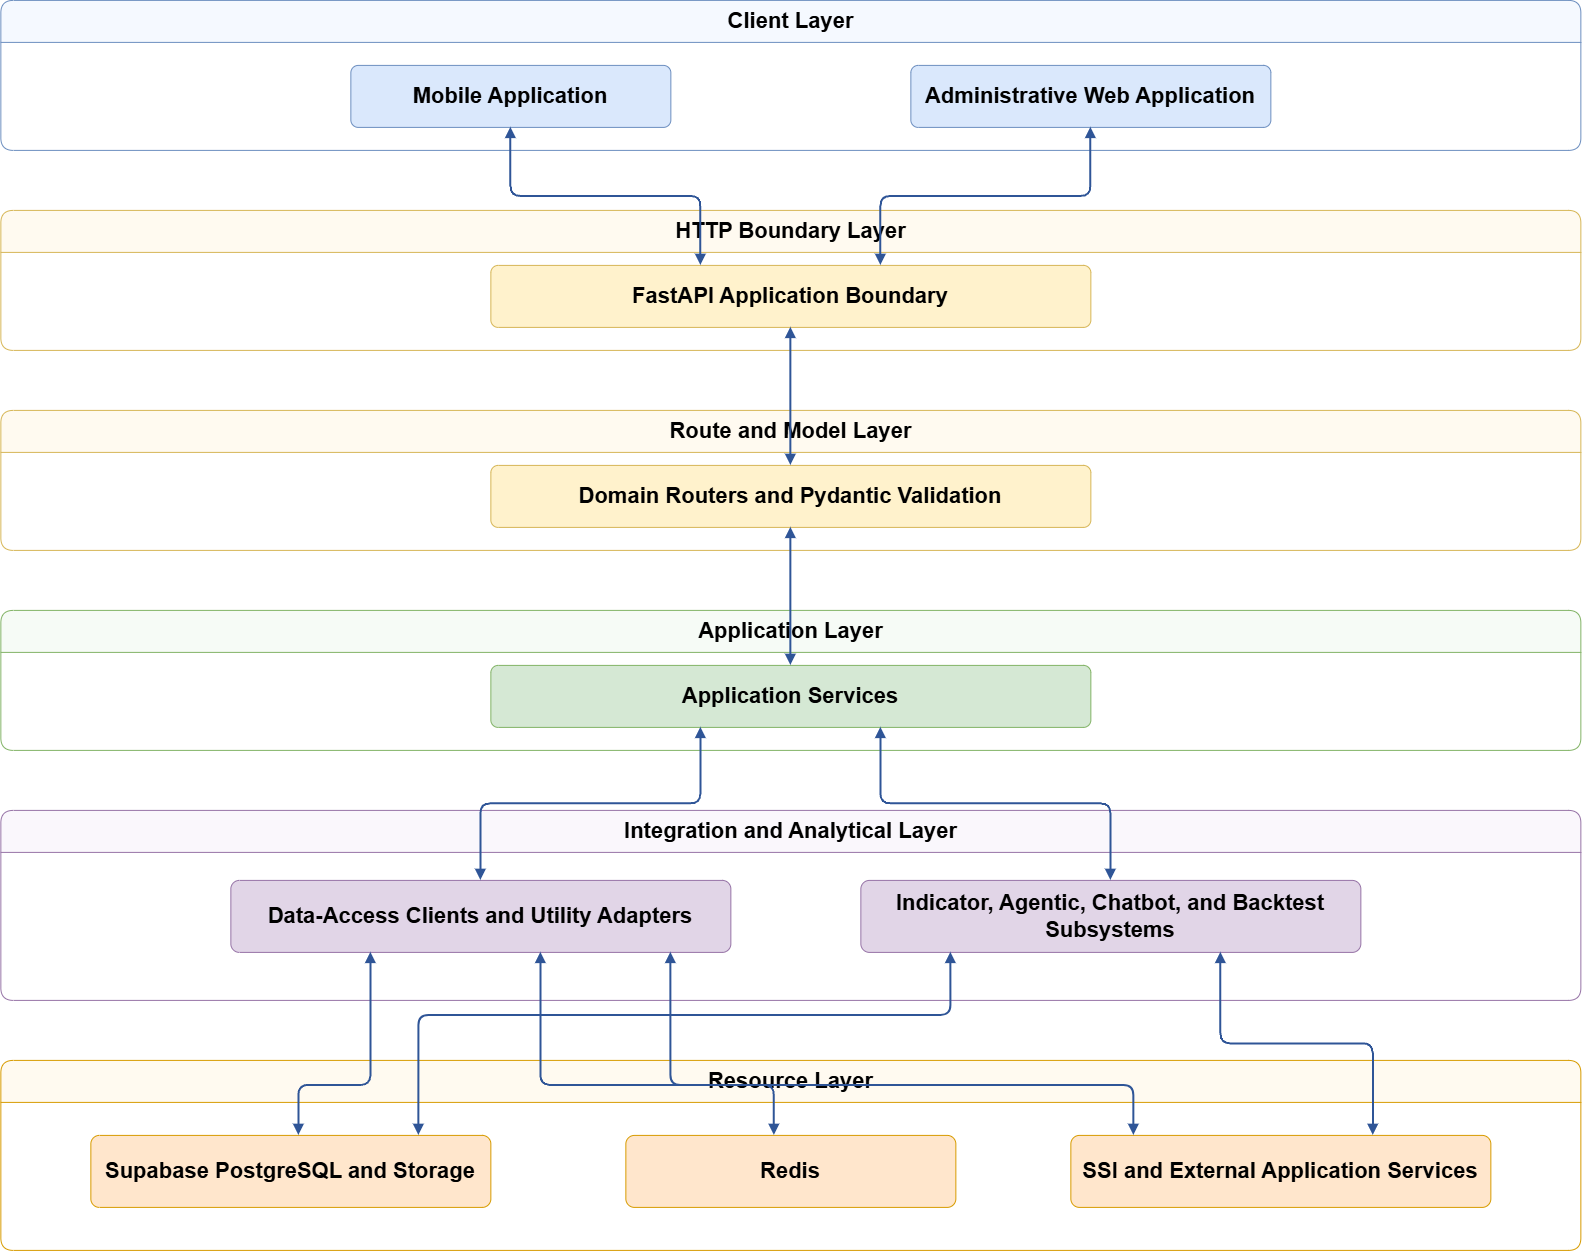
\includegraphics[width=\textwidth,height=0.78\textheight,keepaspectratio]{figures/chapter4/stockrium_backend_layered_design.png}%
    }{%
        \fbox{\parbox[c][5.5cm][c]{0.92\textwidth}{\centering
        Export the Draw.io diagram as\\
        \texttt{figures/chapter4/stockrium\_backend\_layered\_design.png}}}%
    }
    \caption{Layered design of the Stockrium backend service}
    \label{fig:backend-layered-design}
\end{figure}

The layers in Figure~\ref{fig:backend-layered-design} have the following responsibilities:

\begin{itemize}
    \item \textbf{Application boundary.} The FastAPI application registers routers, configures Cross-Origin Resource Sharing (CORS) for allowed browser origins, exposes health endpoints, mounts generated backtest visualizations, and installs common exception handlers. Configuration is loaded from typed environment settings so deployment-specific addresses and credentials are not embedded in route code.
    \item \textbf{Route layer.} Route modules define URL paths, HTTP methods, query and body parameters, access dependencies, and response construction. They remain relatively thin: a route extracts validated values, calls a service, and translates a domain or infrastructure failure into an HTTP result.
    \item \textbf{Model layer.} Pydantic classes describe input and output structures. Once validation succeeds, services receive typed objects rather than unstructured request dictionaries \cite{pydanticModels2026}. These models are particularly important for configurable artificial intelligence (AI) analysis, manual weights, investment-horizon records, authentication, and backtest parameters.
    \item \textbf{Service layer.} Services implement application operations such as obtaining a price series, searching stocks, retrieving financial statements, managing a watchlist entry, calculating technical indicators, running an analysis graph, or maintaining a chat session. A service may combine several tables or providers into one response suited to a user task.
    \item \textbf{Utility and infrastructure layer.} Supabase clients, the direct PostgreSQL connection pool, Redis session operations, SSI FastConnect market-data access, email and Google Identity utilities, model software development kits (SDKs), and Supabase Storage helpers isolate protocol-specific interactions from HTTP routing.
\end{itemize}

This flow is visible in a technical-indicator request. The protected route first obtains the current user from the authentication dependency and validates the requested interval. The market service loads an ordered price series for the symbol, and pandas represents and transforms it as a DataFrame. The technical-indicator service uses the Technical Analysis Library (TA-Lib) to calculate the simple moving average (SMA), exponential moving average (EMA), relative strength index (RSI), moving average convergence divergence (MACD), Bollinger Bands, and stochastic KDJ oscillator. Non-finite warm-up values are converted to \texttt{null} so that the result is valid JavaScript Object Notation (JSON). Finally, the route aligns every indicator value with its trading date and time and returns records suitable for chart rendering. The route does not contain the formulas, and the indicator service does not handle bearer tokens or HTTP status codes.

An AI-analysis request follows the same outer structure but changes at the service boundary. The route validates the analysis configuration and passes the symbol, mode, investment horizon, data-selection switches, and optional weights to the agentic service. The service creates the initial graph state and invokes a compiled LangGraph workflow. Consequently, the HTTP layer is independent of the internal number of specialist agents; later changes to graph routing do not require the mobile request contract to be redesigned.

\subsection{Domain API Modules}
\label{subsec:backend-domain-api-modules}

Routers are divided by application domain instead of by screen. A stock-detail screen can therefore compose calls from the market, company, article, fundamental, and technical modules, while the same modules can be reused by other screens and analytical workflows. Tables~\ref{tab:backend-domain-modules} and~\ref{tab:backend-domain-modules-operational} summarize the modules that belong to the current application.

\begin{table}[htbp]
    \centering
    \caption{Active backend API modules and responsibilities: core data services}
    \label{tab:backend-domain-modules}
    \small
    \setlength{\tabcolsep}{4pt}
    \renewcommand{\arraystretch}{1.22}
    \begin{tabularx}{\textwidth}{>{\raggedright\arraybackslash}p{2.25cm} >{\raggedright\arraybackslash}p{3.35cm} X >{\raggedright\arraybackslash}p{2.45cm}}
        \toprule
        \textbf{Module} & \textbf{Representative interface} & \textbf{Principal responsibility} & \textbf{Main dependency} \\
        \midrule
        Authentication & \texttt{/api/auth/*} & Account creation, email verification, password or Google sign-in, token refresh and revocation, password recovery, and current-user retrieval & Supabase, Redis, Google, Resend \\
        Market and discovery & \texttt{/api/all-stocks}\newline \texttt{/api/price/}\newline \texttt{\{symbol\}}\newline \texttt{/api/market-index}\newline \texttt{/api/investing- idea} & Symbol discovery, current and historical prices, industry movement, index summaries, impact stocks, and deterministic investment-idea lists & Supabase and SSI \\
        Company and fundamentals & \texttt{/api/company/*}\newline \texttt{/api/fundamental-}\newline \texttt{analysis/*} & Company profile, leaders, subsidiaries, financial statements, ratios, stored summaries, and industry aggregates & Supabase \\
        Technical analysis & \texttt{/api/technical-}\newline \texttt{indicators/}\newline \texttt{\{symbol\}} & Load price candles, calculate supported technical-indicator series, align timestamps, and serialize chart-ready values & Market service, pandas, and TA-Lib \\
        Articles & \texttt{/api/articles/*} & Latest, macroeconomic, business, highlighted, category-specific, and stock-specific news retrieval & Supabase \\
        \bottomrule
    \end{tabularx}
\end{table}

\begin{table}[htbp]
    \centering
    \caption{Active backend API modules and responsibilities: user and operational services}
    \label{tab:backend-domain-modules-operational}
    \small
    \setlength{\tabcolsep}{4pt}
    \renewcommand{\arraystretch}{1.22}
    \begin{tabularx}{\textwidth}{>{\raggedright\arraybackslash}p{2.25cm} >{\raggedright\arraybackslash}p{3.35cm} X >{\raggedright\arraybackslash}p{2.45cm}}
        \toprule
        \textbf{Module} & \textbf{Representative interface} & \textbf{Principal responsibility} & \textbf{Main dependency} \\
        \midrule
        Personalization & \texttt{/api/favorite}\newline \texttt{/api/search- history}\newline \texttt{/api/risk- appetite} & User-owned watchlist entries, recent search records, and the selected investment horizon & Supabase and user dependency \\
        Analysis and chat & \texttt{/api/agentic/ analyze}\newline \texttt{/api/agentic/chat}\newline \texttt{/api/agentic/chat/}\newline \texttt{sessions} & Structured stock analysis, stateful conversation, session seeding, history retrieval, and session deletion & LangGraph, model providers, PostgreSQL \\
        Administration and evaluation & \texttt{/api/agentic/}\newline \texttt{admin-analyze}\newline \texttt{/api/agentic/}\newline \texttt{admin-universe/*}\newline \texttt{/api/agentic/ backtest}\newline \texttt{/api/agentic/ backtests} & Role-protected single-symbol or universe analysis, historical pipeline evaluation, and result-artifact listing & Agent graph, backtest services, Supabase Storage \\
        Operations & \texttt{/health}\newline \texttt{/visualizations/*} & Basic process health reporting and delivery of generated backtest visualizations & FastAPI and local artifact directory \\
        \bottomrule
    \end{tabularx}
\end{table}

\FloatBarrier

Authentication is applied through FastAPI dependencies at two levels. Routers containing exclusively protected information---including market, company, fundamental, technical, and article endpoints---declare the current-user dependency once for the entire router. Mixed modules apply the dependency to individual operations. The user dependency verifies the access JSON Web Token (JWT) and also checks that the same token remains present in Redis. This second check enables immediate logout or revocation instead of accepting every cryptographically valid token until its expiry. Administrative operations compose an additional dependency that reads the user's current role from the authoritative \texttt{User} table. A role change therefore takes effect without waiting for a new JWT.

Several services deliberately reuse other domain services. Technical calculation loads candles through the market service instead of implementing a second price-query path. Watchlist and search-history responses enrich stored symbols with profile and current-price information so the mobile client can render useful cards without issuing one request per symbol. Fundamental services resolve a symbol through the \texttt{Stock} relation before obtaining statements and ratios. The agent and chatbot tools also consume the same market, fundamental, technical, and article capabilities used by HTTP routes. Reuse helps keep a value such as the current price or a company identity consistent between a visible screen and an AI response.

\subsection{Request Validation and Response Contract}
\label{subsec:backend-validation-response}

Validation occurs before domain execution whenever an endpoint declares a Pydantic request model. Simple constraints include required fields, numerical bounds, enumerated values, and default settings. Cross-field validation is used when a field cannot be assessed independently. For example, manual AI-analysis weights for news, technical analysis, and fundamental analysis must each be between zero and one, contain no more than two decimal places, and total exactly one after rounding. Backtest parameters bound the maximum holding period, minimum signal score, and lookback window. These checks reduce the chance that invalid configurations reach an expensive model invocation or a long historical simulation.

Validation and normalization are not identical. Pydantic confirms the request shape, while domain services normalize values that carry business meaning. Stock symbols are converted to uppercase before lookup; universe names are stripped and normalized before comparison with \texttt{VN30} and \texttt{VN100}; and Vietnamese chat messages are converted to Unicode Normalization Form C (NFC) before entering the chatbot. The Unicode step is important because visually identical Vietnamese strings can otherwise have different underlying code-point sequences, affecting tokenization, checkpoint content, and comparison behavior.

Client-facing domain endpoints are expected to follow the response envelope shown in Table~\ref{tab:backend-response-envelope}. The envelope separates transport success from the domain payload and gives both clients a stable place to inspect errors. A new universally unique identifier (UUID) is generated for each constructed response. Although the present version does not yet propagate this request identifier through a complete distributed tracing system, it provides a correlation value that can be included in logs and support reports.

\begin{table}[H]
    \centering
    \caption{Standard API response envelope}
    \label{tab:backend-response-envelope}
    \small
    \setlength{\tabcolsep}{6pt}
    \renewcommand{\arraystretch}{1.2}
    \begin{tabular}{p{2.6cm} p{2.3cm} p{7.0cm}}
        \toprule
        \textbf{Field} & \textbf{Type} & \textbf{Meaning} \\
        \midrule
        \texttt{data} & object, array, or scalar & Requested payload on success; normally an empty object when a failure has no safe payload. \\
        \texttt{errorCode} & integer & Zero for a successful operation; a domain-specific nonzero code for failure. \\
        \texttt{errorDesc} & string & Empty on success; a client-readable validation, authorization, lookup, or service error description on failure. \\
        \texttt{requestId} & UUID string & Identifier assigned to the constructed response for correlation and diagnosis. \\
        \texttt{result} & boolean & Indicates whether the requested application operation succeeded. \\
        \bottomrule
    \end{tabular}
\end{table}

The global validation handler intentionally reports HTTP status 400 rather than FastAPI's default 422 response and assigns error code \texttt{400003}. It extracts the first validation failure to keep messages concise for mobile presentation. The common HTTP-exception handler maps frequently used statuses to stable application codes: malformed requests to \texttt{400001}, unauthenticated requests to \texttt{401001}, forbidden requests to \texttt{403001}, missing resources to \texttt{404001}, semantically invalid requests to \texttt{422001}, and server failures to \texttt{500001}. Route-specific response construction may override this general mapping when a more precise domain translation is required. For example, requesting another user's chat session produces a forbidden response, while requesting a nonexistent owned session produces a not-found response.

The response contract also defines a useful client rule: the HTTP status is used for transport and protocol behavior, while \texttt{result}, \texttt{errorCode}, and \texttt{errorDesc} drive application feedback. The mobile HTTP helper can consequently handle authentication failure centrally and still allow a screen to display a domain-specific empty state. Operational endpoints such as \texttt{/health}, the root status route, and mounted static visualization files are intentionally outside the domain envelope because they are consumed as process checks or files rather than application records.

\subsection{Backend Lifecycle, Concurrency, and Failure Containment}
\label{subsec:backend-lifecycle-concurrency}

The backend mixes ordinary data retrieval, asynchronous session operations, numerical indicator calculation, and comparatively slow external model calls. Its lifecycle and concurrency controls therefore aim to reuse expensive resources while bounding fan-out.

The FastAPI process constructs the analysis graph and chatbot graph once when their service module is loaded. A request invokes these compiled graph objects instead of rebuilding nodes, prompts, and persistence configuration for every call. Chat history uses LangGraph checkpoint persistence backed by PostgreSQL \cite{langgraphPersistence2026}. The shared PostgreSQL connection pool is configured with deferred opening and initialized while the chatbot session service ensures the required session table. It maintains between one and ten connections and uses autocommit settings compatible with the Supabase pooler. FastAPI's lifespan handler closes this pool during normal shutdown; an additional process-exit hook covers development shutdown paths in which the Asynchronous Server Gateway Interface (ASGI) lifespan may not complete.

Concurrency is introduced only at bounded points. A normal single-stock request invokes one analysis graph, within which the orchestrator can select and fan out the required specialist branches. Administrative VN30 or VN100 analysis uses a thread pool with four workers. Each worker runs the complete analysis for one symbol, and each future returns either a recommendation or a symbol-specific error record. A temporary provider or data failure for one constituent therefore does not discard successful results for the remainder of the basket. The small fixed pool also prevents an administrative action from issuing dozens of simultaneous language-model calls.

Endpoint definitions use both synchronous and asynchronous functions according to the underlying work. Authentication dependencies and Redis validation are asynchronous because they wait on session input/output (I/O). Many domain services use synchronous Supabase clients or perform numerical work, so their routes are declared as regular functions and can be executed by FastAPI without occupying the event loop as an asynchronous function that performs blocking work would. This arrangement is suitable for the current scale, although very long AI and backtest operations still occupy a request for their full duration. A future production-hardening step could move these operations to a durable job queue and expose progress polling, cancellation, and retry semantics.

Background ingestion is deliberately not scheduled inside the web-process lifecycle. The article updater runs as a separate Railway service, and market-data updaters run as independent worker processes. This separation prevents a weekly news crawl or a continuous market stream from delaying API startup, consuming the web server's request workers, or being duplicated whenever Railway restarts or horizontally scales the API service. The API reads the resulting normalized records from Supabase, while each updater owns its own retry and scheduling behavior.

Failure containment is applied at multiple boundaries. Pydantic rejects malformed requests before service invocation; authentication dependencies stop unauthorized access before domain queries; service methods normalize missing or non-finite data; graph state exposes an error field that the agentic service converts into a runtime failure; and batch analysis records per-symbol exceptions. Global exception handlers then translate uncaught HTTP and validation failures into the common response structure. Finally, the public health route offers a lightweight indication that the FastAPI process is responsive. It is intentionally a liveness check rather than a complete readiness audit: it does not guarantee that Supabase, Redis, SSI, or an AI provider is currently available.

In summary, the backend architecture gives Stockrium one typed and authenticated boundary over heterogeneous data and analytical components. Domain routers define a coherent API, services concentrate reusable application logic, adapters manage infrastructure-specific communication, and lifecycle controls reuse graph and database resources safely. These foundations allow the following sections to describe the agentic workflow and data-processing mechanisms without coupling them to client or HTTP implementation details.

% ============================================================

% ============================================================
\section{Data Architecture and Acquisition Pipelines}
\label{sec:data-architecture-acquisition}

Stockrium depends on data with substantially different lifecycles. User preferences change through application requests; prices change throughout a trading session; financial statements are collected periodically through administrative tools; articles are refreshed weekly; and chatbot checkpoints grow one conversation turn at a time. The data architecture therefore separates persistent relational records, generated file artifacts, short-lived security state, and device-local credentials. It also separates acquisition work from interactive API execution: the mobile application reads normalized data through the backend but does not start a Selenium crawler, an SSI stream, or a news-collection job.

\subsection{Supabase Data Model}
\label{subsec:supabase-data-model}

Supabase PostgreSQL is the principal system of record. PostgreSQL is exposed through Supabase rather than replaced by a proprietary document model, allowing the application to use keys, constraints, relations, pagination, and conflict-aware upserts \cite{supabaseDatabase2026}. Stockrium organizes its application tables into the groups summarized in Table~\ref{tab:supabase-table-groups}. The names shown are the case-sensitive names used by the current backend; quoted identifiers are therefore retained when direct SQL is generated for the chatbot.

\begin{table}[H]
    \centering
    \caption{Principal relational-table groups in Stockrium}
    \label{tab:supabase-table-groups}
    \footnotesize
    \setlength{\tabcolsep}{5pt}
    \renewcommand{\arraystretch}{1.2}
    \begin{tabular}{p{3.0cm} p{9.8cm}}
        \toprule
        \textbf{Data group} & \textbf{Tables and responsibility} \\
        \midrule
        Account and personalization & \texttt{User} stores account identity, credential metadata, and role. \texttt{RiskAppetite} stores the selected investment horizon. \texttt{Favorite} implements the user's stock watchlist. \texttt{Search\_History} stores at most six recent unique stock searches per user. \\
        Market data & \texttt{Stock} is the canonical security directory. \texttt{Stock\_Price\_1m} and \texttt{Stock\_Price\_1d} store OHLCV candles. \texttt{Current\_Stock\_Price} is a latest-quote read model. \texttt{MarketIndex} defines index baskets, \texttt{Current\_Market\_Index} stores the most recent index snapshots, and \texttt{Stock\_MarketIndex} associates securities with indices. \\
        Company and fundamentals & \texttt{BI\_Profile}, \texttt{BI\_Leader}, and \texttt{BI\_Subsidiary} store company description, management, and subsidiary or associate records. \texttt{FA\_Summary}, \texttt{FA\_Indicator}, \texttt{FA\_BalanceSheet}, \texttt{FA\_CashFlow}, and \texttt{FA\_IncomeStatement} store company-level financial evidence. \texttt{FA\_Industry\_Aggregate} stores precomputed annual industry medians and peer counts. \\
        News and classification & \texttt{Article} stores extracted article content, metadata, summary, and sentiment. \texttt{Article\_Stock} and \texttt{Article\_Category} associate articles with securities and categories. \texttt{Category} defines ICB-related groups, while \texttt{Category\_Stock} associates categories with securities. \\
        Chatbot persistence & \texttt{chat\_sessions} records session ownership, title, and timestamps. LangGraph's \texttt{checkpoints}, \texttt{checkpoint\_blobs}, \texttt{checkpoint\_writes}, and \texttt{checkpoint\_migrations} tables persist graph state and checkpoint metadata. \\
        \bottomrule
    \end{tabular}
\end{table}

The central entity is \texttt{Stock}. Company and financial tables use \texttt{stock\_id} to associate a record with a listed security. Annual financial tables conceptually contain one row for a stock and year, while \texttt{FA\_Summary} and \texttt{BI\_Profile} provide stock-level text or profile information. The company can have many leaders and subsidiaries. Price tables currently use a normalized symbol and timestamp as their conflict key; the relationship to \texttt{Stock} is therefore logical through the symbol rather than necessarily enforced by a foreign key.

Account data is separated from market data. \texttt{Favorite} contains only a user--stock association and should not be interpreted as a holding, order, or portfolio position. \texttt{Search\_History} uses the same user and stock identities but applies a recency policy in the service layer. \texttt{RiskAppetite} currently stores one dimension---the selected investment horizon---for each user. These relations let the backend enrich a lightweight personalization record with profile and latest-price information without duplicating company data in each user's rows.

Three explicit join tables represent many-to-many relationships. \texttt{Stock\_MarketIndex} records index constituents, \texttt{Category\_Stock} records the categories to which a stock belongs, and the two article join tables allow one article to be associated with multiple securities or categories without copying the article body. \texttt{FA\_Industry\_Aggregate} is linked to \texttt{Category} by industry identifier and year so a company can be compared with the precomputed median of its peers.

Chat metadata and conversational content are deliberately separated. \texttt{chat\_sessions} maps a client-supplied session identifier to a user and a short title. LangGraph's PostgreSQL saver uses the same session identifier as its thread identifier and stores message-bearing graph states in checkpoint tables \cite{langgraphPersistence2026}. Deleting a conversation removes checkpoint writes, blobs, checkpoints, and then the session record, while the checkpoint-migration table remains framework metadata.

Figure~\ref{fig:stockrium-reduced-erd} presents a reduced entity--relationship view. It intentionally omits most columns and low-level constraints so the important ownership, stock-centered, classification, and conversation relations remain legible.

\begin{figure}[H]
    \centering
    \resizebox{\textwidth}{!}{%
    \begin{tikzpicture}[
        entity/.style={draw, rounded corners=4pt, fill=blue!7, minimum width=3.1cm, minimum height=0.9cm, align=center, font=\small\bfseries},
        group/.style={draw, rounded corners=4pt, fill=green!7, minimum width=4.7cm, minimum height=1.35cm, align=center, font=\scriptsize},
        join/.style={draw, rounded corners=4pt, fill=purple!8, minimum width=3.4cm, minimum height=0.9cm, align=center, font=\scriptsize},
        chat/.style={draw, rounded corners=4pt, fill=orange!9, minimum width=4.2cm, minimum height=1.1cm, align=center, font=\scriptsize},
        rel/.style={-{Latex[length=2.0mm]}, line width=0.6pt, gray!80},
        logical/.style={-{Latex[length=2.0mm]}, line width=0.6pt, dashed, gray!75}
    ]
        \node[entity] (user) at (0,3.2) {\texttt{User}};
        \node[group] (personal) at (4.8,3.2) {\texttt{RiskAppetite}\\\texttt{Favorite}\\\texttt{Search\_History}};
        \node[entity] (stock) at (10.0,3.2) {\texttt{Stock}};
        \node[group] (market) at (15.1,5.2) {\texttt{Stock\_Price\_1m}, \texttt{Stock\_Price\_1d}\\\texttt{Current\_Stock\_Price}};
        \node[group] (company) at (15.1,2.7) {\texttt{BI\_Profile}, \texttt{BI\_Leader}, \texttt{BI\_Subsidiary}\\\texttt{FA\_Summary}, \texttt{FA\_Indicator}\\\texttt{FA\_BalanceSheet}, \texttt{FA\_CashFlow}, \texttt{FA\_IncomeStatement}};
        \node[group] (index) at (10.0,6.1) {\texttt{MarketIndex}\\\texttt{Current\_Market\_Index}};
        \node[join] (stockindex) at (10.0,4.75) {\texttt{Stock\_MarketIndex}};

        \node[entity] (article) at (4.8,-0.5) {\texttt{Article}};
        \node[entity] (category) at (10.0,-0.5) {\texttt{Category}};
        \node[join] (artstock) at (7.4,1.0) {\texttt{Article\_Stock}};
        \node[join] (artcat) at (7.4,-1.7) {\texttt{Article\_Category}};
        \node[join] (catstock) at (12.7,0.7) {\texttt{Category\_Stock}};
        \node[group, minimum width=3.9cm] (industry) at (15.1,-1.2) {\texttt{FA\_Industry\_Aggregate}\\median by category and year};

        \node[chat] (sessions) at (0,-0.3) {\texttt{chat\_sessions}\\session owner and title};
        \node[chat] (checkpoints) at (0,-2.4) {LangGraph checkpoint tables\\state keyed by \texttt{thread\_id}};

        \draw[rel] (user.east) -- node[above, font=\scriptsize] {1:N} (personal.west);
        \draw[rel] (stock.west) -- node[above, font=\scriptsize] {1:N for favorites/searches} (personal.east);
        \draw[rel] (user.south) -- node[right, font=\scriptsize] {1:N} (sessions.north);
        \draw[logical] (sessions.south) -- node[right, font=\scriptsize] {session = thread} (checkpoints.north);

        \draw[logical] (stock.east) to[bend left=18] node[above, font=\scriptsize] {symbol} (market.west);
        \draw[rel] (stock.east) -- node[below, font=\scriptsize] {1:N} (company.west);
        \draw[rel] (stock.north) -- (stockindex.south);
        \draw[rel] (stockindex.north) -- (index.south);

        \draw[rel] (article.north east) -- (artstock.south west);
        \draw[rel] (artstock.north east) -- (stock.south west);
        \draw[rel] (article.south east) -- (artcat.north west);
        \draw[rel] (artcat.north east) -- (category.south west);
        \draw[rel] (category.east) -- (catstock.west);
        \draw[rel] (catstock.north) -- (stock.south east);
        \draw[rel] (category.east) to[bend right=20] node[below, font=\scriptsize] {1:N by year} (industry.west);
    \end{tikzpicture}%
    }
    \caption{Reduced ERD of the principal Stockrium data relationships}
    \label{fig:stockrium-reduced-erd}
\end{figure}

\subsection{Market Price Acquisition Pipeline}
\label{subsec:market-price-acquisition}

The \texttt{update\_stock\_price/} subsystem supports two acquisition modes: historical initialization and daily live operation. Initialization scripts obtain an SSI access token and backfill OHLCV data for stocks in the configured VN-Index universe and for five retained market-index symbols. Daily initialization is divided into 30-day requests because of the upstream API limit and currently loads approximately five years for daily candles. One-minute initialization retrieves the latest 30 days. Rows are normalized into a common \texttt{symbol}, \texttt{trading\_time}, \texttt{open}, \texttt{high}, \texttt{low}, \texttt{close}, and \texttt{volume} representation, deduplicated, and upserted on \texttt{(symbol, trading\_time)}. Requests are paced by approximately 1.1 seconds to reduce SSI rate-limit pressure.

Live acquisition is controlled by a long-running scheduler using Vietnam time (UTC+7). On Monday through Friday, it ensures that three child processes are running from 09:00 inclusive until 15:00 exclusive: a one-minute stock-price stream, a daily stock-price stream, and a market-index stream. The scheduler polls every 30 seconds and restarts a child process if it has exited unexpectedly. At 15:00, it sends an interrupt signal to each stream, waits for a graceful shutdown, and terminates a process only if it does not stop within the timeout.

The one-minute worker subscribes to SSI bar messages, restricts accepted symbols to the configured stock universe and retained indices, and aggregates incoming ticks in an in-memory candle buffer. The key is the pair of symbol and minute. The first tick establishes open, high, low, close, and volume; later ticks update the high and low, replace the close, and accumulate volume. Closed minutes are flushed from a separate loop so network I/O to Supabase does not block the SSI callback. The current open minute is not written during shutdown because it is incomplete.

The daily worker subscribes to the same bar stream but accumulates one current-session record per symbol in \texttt{Stock\_Price\_1d}. Index-bar history is also stored in the 1-minute and daily price tables using the index identifier as the symbol, while index-wide breadth and turnover snapshots arrive through the SSI \texttt{MI} stream and are upserted into \texttt{Current\_Market\_Index} by \texttt{index\_id}. Historical index candles and current index state are therefore separate representations with different query purposes.

At or after 15:05, the scheduler runs three reconciliation jobs exactly once for the date and, importantly, runs them sequentially: one-minute candles, daily candles, and market indices. The one-minute job re-fetches a short two-day lookback and retains 30 days of minute data. The daily job reconciles a three-day lookback and retains five years. The index job retrieves the end-of-day state for the supported indices. Sequential execution prevents three full-universe jobs from making SSI requests simultaneously and exceeding provider limits.

Figure~\ref{fig:market-acquisition-pipeline} summarizes the market-data flow.

\begin{figure}[H]
    \centering
    \resizebox{\textwidth}{!}{%
    \begin{tikzpicture}[
        source/.style={draw, rounded corners=5pt, fill=blue!8, minimum width=3.2cm, minimum height=1.0cm, align=center, font=\small\bfseries},
        process/.style={draw, rounded corners=5pt, fill=green!9, minimum width=3.5cm, minimum height=1.05cm, align=center, font=\small},
        store/.style={draw, rounded corners=5pt, fill=orange!10, minimum width=3.6cm, minimum height=1.0cm, align=center, font=\small\bfseries},
        schedule/.style={draw, rounded corners=5pt, fill=yellow!14, minimum width=3.6cm, minimum height=1.0cm, align=center, font=\small},
        flow/.style={-{Latex[length=2.1mm]}, line width=0.65pt, gray!80}
    ]
        \node[source] (ssiapi) at (0,2.4) {SSI HTTP API\\historical OHLCV};
        \node[source] (ssibar) at (0,0) {SSI WebSocket\\bar stream};
        \node[source] (ssiindex) at (0,-2.4) {SSI WebSocket\\market-index stream};
        \node[source, minimum width=3.8cm] (edgejob) at (0,-4.5) {Scheduled Supabase\\Edge Function job};

        \node[process] (init) at (4.7,2.4) {Initialization\\chunk, normalize, pace};
        \node[process] (minute) at (4.7,0.6) {1-minute buffer\\flush completed candles};
        \node[process] (daily) at (4.7,-0.9) {Daily in-session\\snapshot aggregation};
        \node[process] (indexproc) at (4.7,-2.4) {Index snapshot\\normalization};

        \node[store] (one) at (9.4,1.2) {\texttt{Stock\_Price\_1m}};
        \node[store] (day) at (9.4,-0.4) {\texttt{Stock\_Price\_1d}};
        \node[store] (idx) at (9.4,-2.4) {\texttt{Current\_Market\_Index}};
        \node[store] (currentstock) at (9.4,-4.5) {\texttt{Current\_Stock\_Price}};

        \node[schedule] (scheduler) at (14.1,1.2) {09:00 start\\15:00 stop};
        \node[schedule] (reconcile) at (14.1,-1.4) {15:05 sequential\\1m $\rightarrow$ 1d $\rightarrow$ index};

        \draw[flow] (ssiapi.east) -- (init.west);
        \draw[flow] (init.east) to[bend left=12] (one.west);
        \draw[flow] (init.east) to[bend right=12] (day.west);
        \draw[flow] (ssibar.east) to[bend left=8] (minute.west);
        \draw[flow] (ssibar.east) to[bend right=8] (daily.west);
        \draw[flow] (minute.east) -- (one.west);
        \draw[flow] (daily.east) -- (day.west);
        \draw[flow] (ssiindex.east) -- (indexproc.west);
        \draw[flow] (indexproc.east) -- (idx.west);
        \draw[flow] (edgejob.east) -- node[above, font=\scriptsize] {latest-quote refresh} (currentstock.west);
        \draw[flow] (scheduler.west) -- (one.east);
        \draw[flow] (scheduler.west) -- (day.east);
        \draw[flow] (scheduler.south west) -- (idx.east);
        \draw[flow] (reconcile.west) to[bend left=18] (one.east);
        \draw[flow] (reconcile.west) -- (day.east);
        \draw[flow] (reconcile.west) to[bend right=18] (idx.east);
    \end{tikzpicture}%
    }
    \caption{Historical, live, and post-session market-data acquisition}
    \label{fig:market-acquisition-pipeline}
\end{figure}

The \texttt{Current\_Stock\_Price} table remains important to market lists, favorites, search history, and current-price cards. It is refreshed by scheduled Supabase Edge Function jobs rather than by the Python processes in \texttt{update\_stock\_price/}. This design makes the table a separately maintained latest-quote read model: the Python scheduler owns candle and index-stream persistence, while the managed database-side schedule owns current stock snapshots. Deployment documentation must therefore include both schedules; deploying only the Python service would leave current-price cards dependent on the existing Supabase job.

The scheduler's trading-day test currently recognizes weekdays rather than an exchange-holiday calendar. On a weekday market holiday it may start streams and later execute reconciliation even though no session occurred. Upserts and empty-response handling reduce the risk of corrupting stored candles, but a production version should consume an official Vietnamese exchange calendar.

\subsection{Company and Fundamental Data Pipeline}
\label{subsec:company-fundamental-pipeline}

Company and financial acquisition is an administrative, offline process. It is not invoked from a mobile request because browser automation, file downloads, report parsing, and multi-company imports are too slow and operationally fragile for an interactive API path. The backend serves only data that has already been normalized and stored.

Company-profile collection uses Selenium WebDriver to open SSI iBoard, establish an authenticated browser session, search for a stock, enter dynamically loaded page regions, and parse company information. The crawler obtains profile attributes, leadership records, and subsidiaries or associates. A stock is first resolved through \texttt{Stock}; profile fields are updated in \texttt{BI\_Profile}. Leadership and subsidiary collections are replaced for the stock by deleting their previous rows and inserting the newly observed records. The crawler supports batch operation from symbols already present in \texttt{BI\_Profile} and maintains progress so a long run can resume after a browser or page failure. The use of Selenium for a dynamically rendered source follows the browser-automation rationale introduced in Chapter 2 \cite{seleniumWebDriver2025}.

A separate SSI financial downloader navigates the fundamental-analysis interface and triggers downloads for the balance sheet, income statement, cash-flow statement, and financial-indicator sections. Excel files are converted where necessary, and pandas transforms the downloaded wide layouts into tidy records containing one symbol and financial year per row. Processing removes unnamed or empty columns, normalizes Vietnamese labels into stable database fields, converts numerical values, drops empty trailing years, and serializes missing values as database nulls. The current application schema associates the processed records with \texttt{Stock.id} and stores them in the corresponding \texttt{FA\_*} tables. Upserts use the stock--year identity so rerunning an import corrects or completes existing observations instead of blindly duplicating them. pandas and its workbook engines are suited to this conversion of heterogeneous tabular reports \cite{pandasIO2026}.

Industry aggregation is performed after company profiles and financial indicators are available. The utility maps detailed \texttt{BI\_Profile.icb\_code} values to an ICB industry identifier, groups \texttt{FA\_Indicator} records by industry and year, and computes the median of every available metric while ignoring missing values. It also counts the contributing stocks. Results are upserted into \texttt{FA\_Industry\_Aggregate} on \texttt{(category\_id, year)}. The current utility retains the configured 2021--2025 range and removes obsolete years or invalid category identifiers. Precomputation moves repeated peer aggregation out of user requests and lets the fundamental agent compare a company with a consistent industry benchmark.

Fundamental summaries are also generated as an offline maintenance operation rather than during a mobile request. The active backend reads \texttt{FA\_Summary} by \texttt{stock\_id}. The OpenAI batch utility performs multi-year evidence retrieval, retry, pacing, and skip-existing behavior before persisting the generated text. Its source code retains the earlier name \texttt{fundamental\_analysis\_summary} and earlier lower-case financial-table names; these identifiers refer to the predecessor schema that was later renamed to the active \texttt{FA\_*} tables. They are treated as one logical dataset in this report, with \texttt{FA\_Summary} used consistently as the current name.

Figure~\ref{fig:company-fundamental-pipeline} shows the separation between acquisition, transformation, enrichment, and serving.

\begin{figure}[H]
    \centering
    \resizebox{\textwidth}{!}{%
    \begin{tikzpicture}[
        source/.style={draw, rounded corners=5pt, fill=blue!8, minimum width=3.0cm, minimum height=1.0cm, align=center, font=\small\bfseries},
        process/.style={draw, rounded corners=5pt, fill=green!9, minimum width=3.5cm, minimum height=1.05cm, align=center, font=\small},
        store/.style={draw, rounded corners=5pt, fill=orange!10, minimum width=4.2cm, minimum height=1.0cm, align=center, font=\small},
        flow/.style={-{Latex[length=2.1mm]}, line width=0.65pt, gray!80}
    ]
        \node[source] (iboard) at (0,0) {SSI iBoard\\authenticated pages};
        \node[process] (selenium) at (4.2,1.4) {Selenium crawler\\profile, leaders, subsidiaries};
        \node[process] (download) at (4.2,-1.4) {Selenium downloader\\four financial report types};
        \node[process] (pandas) at (8.6,-1.4) {pandas transformation\\wide reports $\rightarrow$ stock--year rows};
        \node[store] (company) at (8.6,1.4) {\texttt{BI\_Profile}\\\texttt{BI\_Leader}, \texttt{BI\_Subsidiary}};
        \node[store] (financial) at (13.1,-1.4) {\texttt{FA\_Indicator} and\\financial-statement tables};
        \node[process] (median) at (17.4,-1.4) {Industry grouping\\median and peer count};
        \node[store] (aggregate) at (21.7,-1.4) {\texttt{FA\_Industry\_Aggregate}};
        \node[process] (summary) at (17.4,1.4) {Offline OpenAI\\summary generation};
        \node[store] (fasummary) at (21.7,1.4) {\texttt{FA\_Summary}};

        \draw[flow] (iboard.east) to[bend left=15] (selenium.west);
        \draw[flow] (iboard.east) to[bend right=15] (download.west);
        \draw[flow] (selenium.east) -- (company.west);
        \draw[flow] (download.east) -- (pandas.west);
        \draw[flow] (pandas.east) -- (financial.west);
        \draw[flow] (financial.east) -- (median.west);
        \draw[flow] (median.east) -- (aggregate.west);
        \draw[flow] (financial.north east) to[bend left=18] (summary.west);
        \draw[flow] (summary.east) -- (fasummary.west);
    \end{tikzpicture}%
    }
    \caption{Offline company and fundamental-data preparation pipeline}
    \label{fig:company-fundamental-pipeline}
\end{figure}

\subsection{Financial News Pipeline}
\label{subsec:financial-news-pipeline}

The \texttt{update\_articles/} subsystem separates initial collection from periodic refresh. Initial scripts backfill stock-specific, macroeconomic, and category-level news over a longer search horizon and include checkpoint files for resuming multi-page collection. Update scripts request only the latest week and perform one current search page for each configured topic, category, or stock. This distinction reduces the cost of routine updates while preserving a path for initializing a new deployment.

For each target, the pipeline submits a Vietnamese news query to the Serper news endpoint. A result supplies candidate metadata and a source URL. Newspaper3k then downloads the selected page and extracts the article title, body, publication information, and representative image when available. Failed or empty pages are skipped because an inaccessible URL should not produce an article containing only generated text.

The extracted article is passed to \texttt{gpt-4o-mini} with a typed response schema. Stock queries request a short Vietnamese summary and a positive, neutral, or negative label from the perspective of the named security. Category queries use the corresponding industry perspective, while macroeconomic articles receive a general market label. Invalid labels are normalized to neutral before insertion. The original content and source metadata remain in \texttt{Article}, so the summary does not replace the source evidence.

Duplicate prevention occurs at two levels. Existing links are loaded before extraction so a known URL can be skipped without another model call. The insertion path checks again before creating the article. After an article exists, the pipeline checks the relevant join table before inserting \texttt{Article\_Stock} or \texttt{Article\_Category}. The same article can consequently be reused across associations without duplicated content or duplicate join rows. General macroeconomic articles can remain unassociated with an individual security.

The production scheduler uses Vietnam time and executes once per ISO week on Saturday at 23:00. It runs \texttt{update\_macro\_articles.py}, \texttt{update\_category\_articles.py}, and \texttt{update\_stock\_articles.py} sequentially, waiting for each process to finish. A process-local week key prevents a second execution during the same uninterrupted scheduler run. Even if a service restart causes a repeated attempt, link-level duplicate checks make the update substantially idempotent.

\begin{figure}[H]
    \centering
    \resizebox{\textwidth}{!}{%
    \begin{tikzpicture}[
        source/.style={draw, rounded corners=5pt, fill=blue!8, minimum width=3.0cm, minimum height=1.0cm, align=center, font=\small\bfseries},
        process/.style={draw, rounded corners=5pt, fill=green!9, minimum width=3.25cm, minimum height=1.0cm, align=center, font=\small},
        decision/.style={draw, rounded corners=5pt, fill=yellow!13, minimum width=2.8cm, minimum height=1.0cm, align=center, font=\scriptsize},
        store/.style={draw, rounded corners=5pt, fill=orange!10, minimum width=3.5cm, minimum height=1.0cm, align=center, font=\small\bfseries},
        flow/.style={-{Latex[length=2.1mm]}, line width=0.65pt, gray!80}
    ]
        \node[source] (targets) at (0,0) {Macro topics, categories,\\and stock targets};
        \node[process] (serper) at (4.0,0) {Serper News search\\candidate URLs};
        \node[decision] (dup) at (8.0,0) {Link already\\known?};
        \node[process] (newspaper) at (12.1,0) {Newspaper3k\\content extraction};
        \node[process] (openai) at (16.2,0) {OpenAI structured output\\summary and sentiment};
        \node[store] (article) at (20.5,0) {\texttt{Article}};
        \node[store] (joins) at (20.5,-2.2) {\texttt{Article\_Stock} or\\\texttt{Article\_Category}};
        \node[process, fill=yellow!10] (schedule) at (0,-2.2) {Saturday 23:00 VN\\macro $\rightarrow$ category $\rightarrow$ stock};
        \node[process, fill=gray!8] (skip) at (8.0,-2.2) {Skip duplicate\\without another model call};

        \draw[flow] (targets.east) -- (serper.west);
        \draw[flow] (serper.east) -- (dup.west);
        \draw[flow] (dup.east) -- node[above, font=\scriptsize] {no} (newspaper.west);
        \draw[flow] (newspaper.east) -- (openai.west);
        \draw[flow] (openai.east) -- (article.west);
        \draw[flow] (article.south) -- (joins.north);
        \draw[flow] (dup.south) -- node[right, font=\scriptsize] {yes} (skip.north);
        \draw[flow] (schedule.north) -- (targets.south);
    \end{tikzpicture}%
    }
    \caption{Initial and weekly financial-news processing flow}
    \label{fig:financial-news-pipeline}
\end{figure}

The article updater is deployed as a separate Railway service rather than as an in-process FastAPI job. This separation prevents a crawl and a sequence of model calls from delaying API requests or being duplicated for every web-server worker. It also allows the updater container to install the native parsing dependencies required by Newspaper3k independently of the main backend image.

\subsection{Storage Responsibilities}
\label{subsec:storage-responsibilities}

Not every value belongs in the relational database. Table~\ref{tab:storage-responsibility-boundaries} distinguishes the four storage mechanisms used by Stockrium and clarifies which copy is authoritative.

\begin{table}[H]
    \centering
    \caption{Storage responsibility boundaries}
    \label{tab:storage-responsibility-boundaries}
    \footnotesize
    \setlength{\tabcolsep}{5pt}
    \renewcommand{\arraystretch}{1.2}
    \begin{tabular}{p{2.8cm} p{5.1cm} p{5.0cm}}
        \toprule
        \textbf{Storage} & \textbf{Stored information} & \textbf{Responsibility and lifecycle} \\
        \midrule
        Supabase PostgreSQL & Accounts, personalization, security directory, market candles and snapshots, company profiles, financial records, industry aggregates, articles, classifications, chat-session metadata, and LangGraph checkpoints & Authoritative durable relational data. Accessed through Supabase PostgREST for domain services and through pooled PostgreSQL connections for checkpointing and controlled chatbot queries. \\
        Supabase Storage & Manually uploaded JSON backtest reports in the \texttt{backtests} bucket & Durable object artifacts that are listed by the backend and opened by the administrative dashboard. The storage helper supports replacement upload and public-URL generation, but the current backtest execution route does not upload automatically. \\
        Redis & Access token, refresh token, verification or reset OTP, attempt counter, resend cooldown state, and one-time reset-session mappings & Expiring server-side security state. Enables token revocation and automatic removal through TTL; it is not a source of permanent user or financial records \cite{redisDataTypes2026}. \\
        Expo SecureStore & Mobile access token and refresh token; also small local preferences such as onboarding completion, theme, language, and saved analysis configuration & Device-local encrypted key--value state. Tokens are removed when refresh fails or the user signs out. The backend remains authoritative for accounts and sessions \cite{expoSecureStore2026}. \\
        \bottomrule
    \end{tabular}
\end{table}

Backtest execution returns its result to the administrative workflow, where the JSON artifact can be inspected or exported. Upload to the \texttt{backtests} bucket is a separate manual administrative action. Once an artifact has been uploaded, the backend storage helper lists the available JSON files and produces the public URLs used by the dashboard. This distinction prevents the presence of an upload helper from being mistaken for an automatic persistence step in every backtest request.

Redis key namespaces reflect these responsibilities. Access and refresh sessions use \texttt{session:access:\{user\_id\}} and \texttt{session:refresh:\{user\_id\}} with configurable token lifetimes. OTP values use \texttt{otp:\{purpose\}:\{email\}}, while \texttt{otp:attempts:\{purpose\}:\{email\}} counts failed verification attempts under the same expiry. The default OTP validity is ten minutes with a maximum of five attempts. A successful password-reset verification produces a five-minute one-time reset session and an email-to-session reverse mapping so an older session can be invalidated.

The mobile application stores the access and refresh tokens under \texttt{access\_token} and \texttt{refresh\_token} in SecureStore. It does not store a durable copy of favorites, risk horizon, chat history, or financial records as an authoritative local database. Those values are requested from the backend. This boundary prevents a device preference or stale cache from being mistaken for a confirmed server-side state.

The acquisition pipelines and storage boundaries together provide a stable evidence layer for the analytical components. Live and offline processes normalize heterogeneous sources before they reach application services; relational links preserve stock, industry, article, and user context; and short-lived secrets remain outside durable business tables. The next section builds the agentic stock-analysis design on top of these prepared data products.

% ============================================================

% ============================================================
\section{Agentic Stock Analysis Design}
\label{sec:agentic-stock-analysis-design}

The principal analytical feature of Stockrium is implemented as a stateful directed graph rather than as one monolithic language-model prompt. The graph separates planning, evidence preparation, specialist analysis, synthesis, and deterministic post-processing. This separation is important because the three evidence domains have different structures: price series require numerical calculation, financial statements require multi-year and industry-aware comparison, and articles require relevance filtering and qualitative interpretation. Treating them as independent branches also makes it possible to disable selected evidence, diagnose a weak branch, and reuse the same components in live analysis and historical evaluation.

LangGraph provides the state-graph abstraction used to declare nodes, edges, shared state, and parallel branches \cite{langgraph2026graphapi}. The language model is used where semantic interpretation or natural-language synthesis is required, while Python functions retain control over interval selection, indicator calculation, technical scoring, confidence calculation, veto conditions, and price-boundary enforcement. The resulting design is therefore hybrid: it benefits from the explanatory ability of a language model without assigning every numerical or safety-sensitive decision to generated text.

\subsection{Graph Topology and Shared State}
\label{subsec:analysis-graph-state}

The compiled analysis graph contains five nodes: an orchestrator, three specialist branches, and an aggregator. Figure~\ref{fig:analysis-graph-topology} presents the execution topology. After the orchestrator creates a plan, LangGraph activates the article, fundamental, and technical nodes from the same state. Each branch writes its own entry into the shared result dictionary. The dictionary uses a merge reducer, so branch updates are combined rather than allowing the last completed branch to replace earlier results. The aggregator is executed only after the specialist branches have reached their outgoing edges.

\begin{figure}[H]
    \centering
    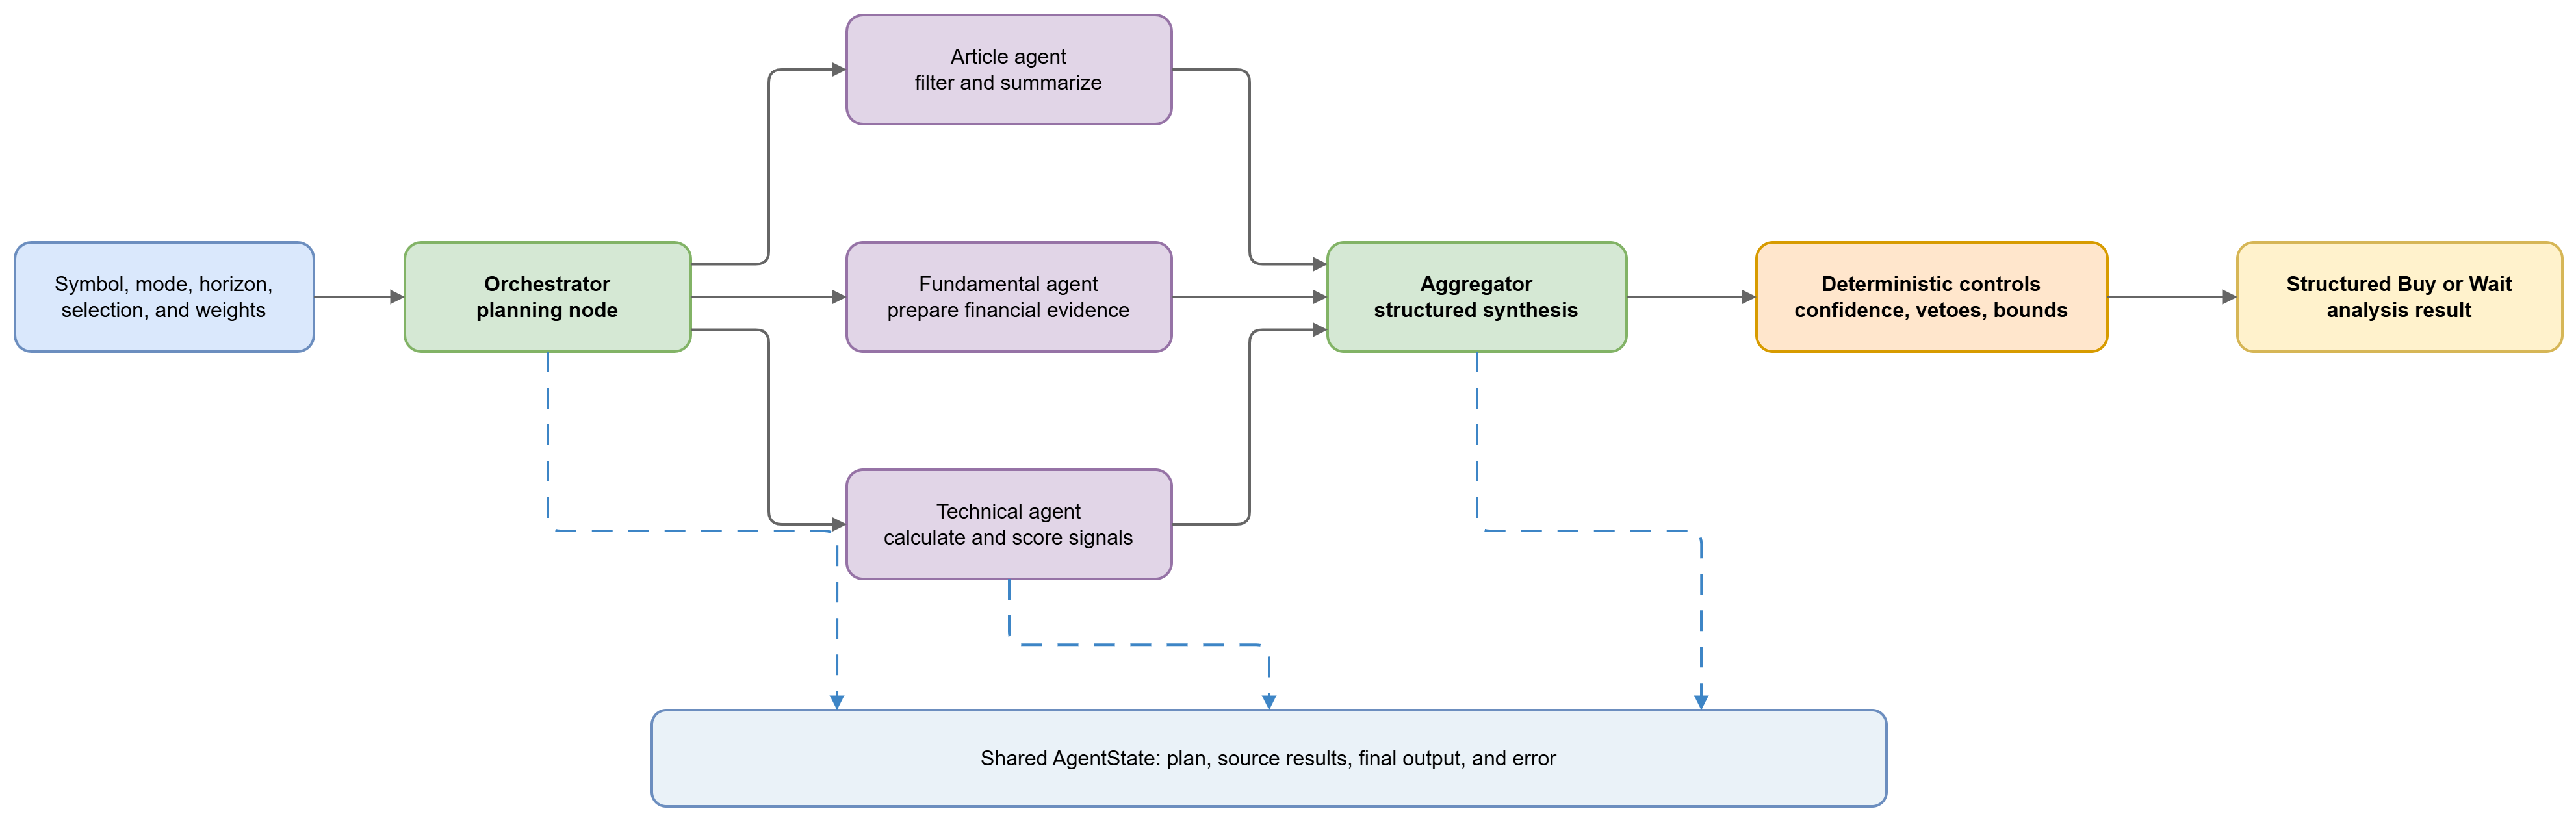
\includegraphics[width=\textwidth,keepaspectratio]{diagrams/chapter4/stockrium_agent_topology.png}
    \caption{Execution topology of the Stockrium analysis graph}
    \label{fig:analysis-graph-topology}
\end{figure}

The shared \texttt{AgentState} is a typed dictionary containing the fields summarized in Table~\ref{tab:analysis-agent-state}. State is the contract between graph nodes: a node reads only the context it requires and returns only the fields it changes. The graph can consequently add or replace a specialist without redesigning the public HTTP request.

\begin{table}[H]
    \centering
    \caption{Principal fields in the analysis graph state}
    \label{tab:analysis-agent-state}
    \small
    \setlength{\tabcolsep}{5pt}
    \renewcommand{\arraystretch}{1.18}
    \begin{tabular}{p{3.0cm} p{3.0cm} p{6.5cm}}
        \toprule
        \textbf{Field} & \textbf{Producer} & \textbf{Purpose} \\
        \midrule
        \texttt{mode} & API service & Distinguishes automatic and manual analysis; the state type also permits reuse by chat-related execution. \\
        \texttt{user\_input} & API service & Vietnamese task statement supplied to planning and final synthesis. \\
        \texttt{risk\_appetite} & API service & Contains the user's selected investment horizon, which drives time scale, default weights, and numerical bounds. \\
        \texttt{symbol} & API service & Identifies the Vietnamese listed stock being analyzed. \\
        \texttt{data\_selection} & API service & Contains enabled news, technical indicators, fundamental groups, and optional manual weights. \\
        \texttt{plan} & Orchestrator & Supplies date ranges and the deterministic technical interval to specialist nodes. \\
        \texttt{agent\_results} & Specialist nodes & Merged dictionary containing separate article, fundamental, and technical evidence. \\
        \texttt{final\_output} & Aggregator & Structured recommendation, scores, confidence, explanations, and conditional risk values. \\
        \texttt{error} & Any terminal failure & Carries a pipeline error back to the application service. \\
        \bottomrule
    \end{tabular}
\end{table}

Automatic and manual requests enter the same graph. In automatic mode, the application service replaces the submitted selection with an empty configuration; selection normalization interprets every missing switch as enabled and applies horizon-based default weights. In manual mode, the user's switches and weights remain in the state. All three graph branches are still reached structurally, but a disabled branch returns a clear disabled-source marker instead of performing unnecessary data interpretation or model work. This approach keeps the topology stable while making behavior configurable.

\subsection{Orchestration and Horizon-Aware Planning}
\label{subsec:analysis-orchestrator-planning}

The orchestrator converts the request and horizon into a structured plan. It calls \texttt{gpt-4o-mini} with temperature zero and parses the response into a Pydantic \texttt{OrchestratorPlan}. Structured output is preferable to parsing arbitrary prose because both the article and technical branches require valid \texttt{YYYY-MM-DD} boundaries \cite{openaiStructuredOutputs2026}. The prompt defines a recent lookback of approximately 60 days for short-term analysis, 180--365 days for medium-term analysis, and at least 730 days for long-term analysis. The end date is the current date.

The model does not choose the candle interval. After parsing the generated dates, Python overwrites the technical interval according to the normalized investment horizon. Short-term requests use daily candles, medium-term requests use weekly candles, and long-term requests use monthly candles. If the horizon is absent or unrecognized, the system defaults to the medium-term configuration. This deterministic mapping prevents prompt variation from assigning inconsistent analytical scales to users with the same horizon.

The fundamental branch is intentionally not given a horizon-specific number of financial years. It examines up to the five latest annual periods regardless of whether the user selected a short-, medium-, or long-term profile. This asymmetry is deliberate: the horizon changes the sensitivity of price signals, but company quality should not be inferred from a single recent accounting period. The aggregator later changes the relative influence of the fundamental evidence according to the horizon.

\subsection{Specialist Evidence Agents}
\label{subsec:analysis-specialist-agents}

The specialist nodes do not all use the language model in the same way. The technical node is primarily deterministic, the fundamental node prepares a structured textual evidence package without making the final recommendation, and the article node uses a model to filter and summarize natural-language news. Table~\ref{tab:specialist-agent-responsibilities} highlights these differences.

\begin{table}[H]
    \centering
    \caption{Responsibilities and outputs of specialist analysis nodes}
    \label{tab:specialist-agent-responsibilities}
    \small
    \setlength{\tabcolsep}{4pt}
    \renewcommand{\arraystretch}{1.2}
    \begin{tabular}{p{2.45cm} p{3.2cm} p{4.8cm} p{2.6cm}}
        \toprule
        \textbf{Node} & \textbf{Evidence} & \textbf{Processing} & \textbf{Branch output} \\
        \midrule
        Technical & Historical OHLCV candles and the most recent available price & Indicator calculation, latest-versus-previous comparison, deterministic binary scoring, and missing-value sanitation & Indicator values, explanations, current price, \texttt{total\_score}, and \texttt{max\_score} \\
        Fundamental & Annual financial indicators, statements, company profile, ICB classification, and precomputed industry medians & Five-year ordering, CAGR, DuPont preparation, sector-specific metric selection, and industry comparison & Evidence text organized by financial category \\
        Article & Stored articles related to the symbol within the planned dates & Date filtering, compact evidence construction, relevance screening, and model-based summary of benefits and risks & Vietnamese news summary or an explicit no-data marker \\
        \bottomrule
    \end{tabular}
\end{table}

\subsubsection{Technical-Analysis Agent}
\label{subsubsec:technical-analysis-agent}

The technical agent first obtains the most recent one-minute price when live analysis is being performed. It separately loads candles in the horizon-selected interval and date range. Daily records are aggregated by the market service when weekly or monthly analysis is requested. The indicator service calculates moving averages, RSI, Bollinger Bands, MACD, and KDJ. During backtesting, the same node can use a historical indicator source and suppress current-price lookup so that a future price is not introduced into a past decision.

Each enabled indicator contributes at most one point. The scoring rules are shown in Table~\ref{tab:technical-signal-scoring}. They focus on a positive transition or strengthening condition rather than assigning a point whenever an indicator has any valid value. A missing indicator receives zero and an explanatory reason. The denominator is the number of indicators enabled by the user, not a fixed value of five, which keeps the later 60\% threshold meaningful in manual mode.

\begin{table}[H]
    \centering
    \caption{Deterministic positive-signal conditions in the technical agent}
    \label{tab:technical-signal-scoring}
    \footnotesize
    \setlength{\tabcolsep}{4pt}
    \renewcommand{\arraystretch}{1.18}
    \begin{tabular}{p{1.65cm} p{10.9cm}}
        \toprule
        \textbf{Indicator} & \textbf{One-point condition; satisfying any listed condition is sufficient} \\
        \midrule
        RSI & Crosses upward through 50; is between 50 and 70 and rising; or is below 35 but recovering from the previous value. \\
        Moving averages & SMA20 crosses upward through SMA50; SMA20 remains above SMA50 with an expanding positive gap; or current price is above SMA20 while SMA20 is above SMA50. \\
        Bollinger Bands & Price crosses upward through the middle band; remains above the middle band with a widening positive distance; or recovers while at or below the lower band. \\
        MACD & MACD crosses upward through its signal line; MACD is above the signal while the histogram strengthens; or the histogram changes from negative to nonnegative. \\
        KDJ & K crosses upward through D; K is above D while J strengthens; or K rises while below 20. \\
        \bottomrule
    \end{tabular}
\end{table}

For every enabled indicator, the output contains current and previous values, a binary score, and a rule-generated reason. The agent also returns the actual covered dates, number of candles, interval, and display price. The aggregator can therefore ask the language model to explain concrete signals while retaining a score that was produced outside the model. Overbought RSI, price above the upper Bollinger Band, weakening MACD histogram, or overbought KDJ can be described as cautionary evidence even though the system's recommendation vocabulary remains limited to Buy and Wait.

\subsubsection{Fundamental-Analysis Agent}
\label{subsubsec:fundamental-analysis-agent}

The fundamental agent loads financial indicators, income statements, cash flows, a stored summary, and company-profile metadata. It retains up to five most recent annual records and orders them chronologically. For applicable values it computes compound annual growth rate as

\begin{equation}
    \operatorname{CAGR}(x) = \left(\frac{x_{n}}{x_{0}}\right)^{\frac{1}{y_{n}-y_{0}}} - 1,
    \label{eq:fundamental-cagr}
\end{equation}

where $x_{0}$ and $x_{n}$ are the earliest and latest positive observations and $y_{n}-y_{0}$ is the elapsed number of years. CAGR is omitted when fewer than two valid points exist, the elapsed period is nonpositive, or either endpoint is nonpositive. This restriction avoids producing a misleading growth percentage for a series that changes sign.

For nonfinancial firms, selected evidence is organized into liquidity, leverage, efficiency, profitability, and valuation. The leverage or profitability preparation can include a DuPont decomposition,

\begin{equation}
    ROE = \text{Net Margin} \times \text{Asset Turnover} \times \text{Financial Leverage},
    \label{eq:dupont-stockrium}
\end{equation}

which helps distinguish margin-driven returns from efficient asset use or debt-supported returns. For firms whose ICB code begins with 8, the agent uses a financial-sector presentation based on available CAMELS-related measures. It avoids relying on P/E and EV/EBITDA for financial-sector valuation and instead presents P/B. When specialized measures such as CAR, NPL, NIM, LDR, or CIR are unavailable, the evidence explicitly states the limitation rather than filling it with an inferred value.

The company is also compared with precomputed annual medians for the corresponding ICB industry. A comparison table is included only when at least three peers contribute, reducing the risk of treating one or two companies as a representative benchmark. The evidence includes the latest company value, latest industry median, company CAGR, and industry CAGR for selected measures. These deterministic preparations give the aggregator concrete relative context rather than asking it to decide what constitutes the industry from an unrestricted prompt.

Disabling every fundamental category causes the branch to return an explicit disabled marker. Data-access failures and completely missing financial records are converted to a no-data marker and do not terminate the other branches. This is important for newly listed companies and for batch analysis, where one incomplete company should not cancel an entire universe.

\subsubsection{Article-Analysis Agent}
\label{subsubsec:article-analysis-agent}

The article agent retrieves records already associated with the selected stock and filters them to the orchestrator's date interval. Its input to the model contains each article's date, title, available summary, and stored sentiment. The model is instructed to retain useful and relevant content and return a Vietnamese structure containing the main information, positive points, and negative points or risks. This branch uses a low but nonzero temperature of 0.2 because limited linguistic variation is acceptable in a summary, while highly variable creative output is undesirable in financial analysis.

If the user disables news, no article falls within the planned period, or the branch cannot provide usable content, it returns a recognizable marker. The aggregator detects these markers in Python. Missing news is therefore treated as absent evidence rather than silently converted into neutral evidence that would still affect confidence.

\subsection{Aggregation and Structured Recommendation}
\label{subsec:analysis-aggregation}

The aggregator receives the three branch results and first determines which sources contain real evidence. Technical data is active only if the result is a dictionary containing indicators and no error. Fundamental and article text are active only if they are nonempty and do not contain known disabled or no-data markers. These flags are placed into the aggregation prompt so the model cannot legitimately fill an absent section with invented analysis.

The model parses its response into an \texttt{InvestmentRecommendation} schema. The schema restricts the recommendation to \textit{Mua} (Buy) or \textit{Chờ} (Wait); requires separate technical, fundamental, news, and summary explanations; and carries the raw labels needed by deterministic confidence calculation. It also permits entry, take-profit, stop-loss, and maximum-holding values only for a candidate Buy result. A structured schema guarantees field presence and type conformance, but it does not by itself guarantee factual correctness. Stockrium therefore applies Python post-processing after parsing.

The aggregator's prompt requires technical explanations to cover each enabled indicator, fundamental explanations to use the appropriate nonfinancial or financial-sector structure, and news explanations to distinguish macro-level, company-level, and outlook implications. It also instructs the model not to repeat the recommendation or invent confidence inside narrative fields. If generation reaches the configured output-token limit, the aggregator retries once with an instruction to shorten each explanation. Any unrecovered aggregation exception places an error in graph state and produces a safe Wait-shaped fallback with empty risk values.

\subsection{Deterministic Confidence and Decision Controls}
\label{subsec:analysis-deterministic-controls}

Confidence is calculated after structured parsing and must not be interpreted as a probability of future profit. Let $s_t$ be the technical score and $m_t$ the number of enabled technical indicators. The normalized source components are

\begin{equation}
    c_t = \frac{s_t}{m_t}, \qquad
    c_f \in \{1, 0.5, 0\}, \qquad
    c_n \in \{1, 0.5, 0\},
    \label{eq:confidence-components}
\end{equation}

where fundamental labels \texttt{strong}, \texttt{neutral}, and \texttt{weak} map respectively to $1$, $0.5$, and $0$, while article labels \texttt{positive}, \texttt{neutral}, and \texttt{negative} use the same mapping. If no technical indicator is enabled, the technical component is set to $0$; in that configuration the technical source is inactive and is removed by the effective-weight renormalization in Equation~\ref{eq:effective-confidence}, so this value does not affect the final confidence.

Default weights vary by horizon as shown in Table~\ref{tab:confidence-horizon-weights}. The short-term profile emphasizes price signals, while the long-term profile emphasizes company fundamentals. Manual weights replace this table after API validation has established that the three values are within $[0,1]$ and total one.

\begin{table}[H]
    \centering
    \caption{Default confidence weights by investment horizon}
    \label{tab:confidence-horizon-weights}
    \small
    \renewcommand{\arraystretch}{1.2}
    \begin{tabular}{lccc}
        \toprule
        \textbf{Horizon} & \textbf{Technical} & \textbf{Fundamental} & \textbf{News} \\
        \midrule
        Short term: below 3 months & 0.60 & 0.10 & 0.30 \\
        Medium term: 3--12 months & 0.40 & 0.40 & 0.20 \\
        Long term: above 1 year & 0.15 & 0.70 & 0.15 \\
        \bottomrule
    \end{tabular}
\end{table}

An unavailable or disabled source is removed before aggregation. If $A$ is the set of active sources and $w_i$ is the default or manual base weight, the effective weight is

\begin{equation}
    w_i^{\prime} =
    \begin{cases}
        \displaystyle\frac{w_i}{\sum_{j \in A} w_j}, & i \in A,\\[6pt]
        0, & i \notin A,
    \end{cases}
    \qquad
    C = \sum_i w_i^{\prime}c_i.
    \label{eq:effective-confidence}
\end{equation}

Thus, disabling news does not leave its original weight as an invisible neutral contribution. The remaining evidence is renormalized to sum to one. The response exposes the component scores, effective weights, raw technical score, qualitative labels, final confidence, and the fixed acceptance threshold of $0.55$, making the calculation inspectable.

The decision layer acts conservatively as a veto system. The model is first instructed to apply the same rules and generates a candidate recommendation. Python never promotes a model-generated Wait to Buy; it can only preserve a candidate Buy or downgrade it. A candidate Buy is changed to Wait when any applicable condition holds:

\begin{itemize}
    \item the technical score is below $\lceil 0.60m_t \rceil$, provided at least one technical indicator is enabled;
    \item fundamental evidence exists and its label is \texttt{weak};
    \item news evidence exists and its label is \texttt{negative}; or
    \item deterministic confidence is below $0.55$.
\end{itemize}

If fundamental or news evidence is absent, its veto is skipped rather than treated as a negative signal. If the final result is Wait, all trading-plan values are set to \texttt{null}. This long-only design prevents the result from resembling a short-sale or execution instruction and is consistent with the application scope.

For a surviving Buy result, the current technical price is used when the model does not supply an entry price. Python then constrains take-profit distance, stop-loss distance, and maximum holding count according to Table~\ref{tab:horizon-price-boundaries}. An out-of-range value is clamped to the nearest boundary; a missing or invalid value is replaced by the midpoint of the permitted range. Final prices are recalculated from the bounded percentages and appended to the narrative summary only after enforcement, preventing the displayed text from disagreeing with the structured numerical fields.

\begin{table}[H]
    \centering
    \caption{Implemented horizon-specific trading-plan boundaries}
    \label{tab:horizon-price-boundaries}
    \small
    \setlength{\tabcolsep}{7pt}
    \renewcommand{\arraystretch}{1.2}
    \begin{tabular}{lccc}
        \toprule
        \textbf{Horizon} & \textbf{Take-profit distance} & \textbf{Stop-loss distance} & \textbf{Maximum hold} \\
        \midrule
        Short term & 8--15\% above entry & 4--7\% below entry & 5--15 candles \\
        Medium term & 15--30\% above entry & 7--12\% below entry & 15--60 candles \\
        Long term & 40--80\% above entry & 15--20\% below entry & 120--260 candles \\
        \bottomrule
    \end{tabular}
\end{table}

Two implementation qualifications are necessary for an accurate description. First, the prompt asks the model to maintain a reward-to-risk ratio of at least 1.5, but the current Python post-processing does not recalculate this condition as a final veto after clamping. The ratio displayed in the result is therefore informative rather than a deterministically guaranteed constraint. Second, the boundary configuration describes maximum hold in daily-candle terms, while live technical analysis maps medium- and long-term horizons to weekly and monthly candles and the mobile interface labels the field as a number of candles. The present code does not convert the bounded count between these time scales. Consequently, the values in Table~\ref{tab:horizon-price-boundaries} document the implementation but should not be reinterpreted as a universally consistent calendar duration. Aligning interval semantics and adding a final reward-to-risk assertion are appropriate hardening tasks for future work.

Overall, the agentic workflow separates evidence acquisition and deterministic calculation from semantic synthesis. Parallel specialist nodes make each analytical perspective inspectable; structured models constrain generated objects; and Python checks can reject a candidate Buy that violates measurable rules. The workflow remains an analytical support mechanism rather than an autonomous trading system: it supplies a traceable Buy-or-Wait assessment, but it neither places an order nor guarantees an investment outcome.

% ============================================================

% ============================================================
\chapter*{References}
\phantomsection
\addcontentsline{toc}{chapter}{References}
\begin{thebibliography}{99}
\bibitem{vsdc2025}
Vietnam Securities Depository and Clearing Corporation, ``Securities account statistics,'' 2025. [Online]. Available: \url{https://www.vietnam.vn/en/thi-truong-chung-khoan-viet-nam-co-hon-11-trieu-tai-khoan-giao-dich}.

\bibitem{vinacapital2024}
VinaCapital, ``Vietnam's Resilient Stock Market,'' Insights Report, 2024. [Online]. Available: \url{https://vinacapital.com/wp-content/uploads/2024/07/VinaCapital-Insights-Vietnams-Resilient-Stock-Market.pdf}.

\bibitem{barberOdean2013}
B. M. Barber and T. Odean, ``The behavior of individual investors,'' in \textit{Handbook of the Economics of Finance}, vol. 2B, G. M. Constantinides, M. Harris, and R. M. Stulz, Eds. Elsevier, 2013, pp. 1533--1570.

\bibitem{wu2023bloomberggpt}
S. Wu et al., ``BloombergGPT: A large language model for finance,'' arXiv preprint arXiv:2303.17564, 2023.

\bibitem{yang2023fingpt}
H. Yang, X.-Y. Liu, and C. D. Wang, ``FinGPT: Open-source financial large language models,'' arXiv preprint arXiv:2306.06031, 2023.

\bibitem{xiao2024tradingagents}
Y. Xiao, E. Sun, D. Luo, and W. Wang, ``TradingAgents: Multi-agents LLM financial trading framework,'' arXiv preprint arXiv:2412.20138, 2024.

\bibitem{yu2023finmem}
Y. Yu, H. Li, Z. Chen, Y. Jiang, Y. Li, D. Zhang, R. Liu, J. W. Suchow, and K. Khashanah, ``FinMem: A performance-enhanced LLM trading agent with layered memory and character design,'' arXiv preprint arXiv:2311.13743, 2023.

\bibitem{araci2019finbert}
D. Araci, ``FinBERT: Financial sentiment analysis with pre-trained language models,'' arXiv preprint arXiv:1908.10063, 2019.

\bibitem{halder2022finbertlstm}
S. Halder, ``FinBERT-LSTM: Deep learning based stock price prediction using news sentiment analysis,'' arXiv preprint arXiv:2211.07392, 2022.

\bibitem{tung2021phobert}
N. S. Tung, N. N. Long, T. Tran, N. T. Thao, D. T. T. Phuong, and T. Nguyen, ``Stock article title sentiment-based classification using PhoBERT,'' in \textit{Proceedings of the 2nd International Conference on Human-centered Artificial Intelligence}, CEUR Workshop Proceedings, vol. 3026, pp. 225--233, 2021. [Online]. Available: \url{https://ceur-ws.org/Vol-3026/paper25.pdf}.

\bibitem{vu2023sentiments}
L. T. Vu, D. N. Pham, H. T. Kieu, and T. T. T. Pham, ``Sentiments extracted from news and stock market reactions in Vietnam,'' \textit{International Journal of Financial Studies}, vol. 11, no. 3, art. 101, 2023, doi: 10.3390/ijfs11030101.

\bibitem{truong2022lstm}
C.-D. Truong, D.-Q. Tran, V.-D. Nguyen, H.-T. Tran, and T.-D. Hoang, ``Predicting Vietnamese stock market using the variants of LSTM architecture,'' in \textit{Nature of Computation and Communication}, Lecture Notes of the Institute for Computer Sciences, Social Informatics and Telecommunications Engineering. Springer, 2022, doi: 10.1007/978-3-030-92942-8\_11.

\bibitem{phuoc2024ml}
T. Phuoc, P. T. K. Anh, P. H. Tam, and C. V. Nguyen, ``Applying machine learning algorithms to predict the stock price trend in the stock market: The case of Vietnam,'' \textit{Humanities and Social Sciences Communications}, vol. 11, art. 393, 2024, doi: 10.1057/s41599-024-02807-x.

\bibitem{son2025deepmodels}
H. H. Son, N. T. Phuong, N. T. Linh, and P. T. Loan, ``A comprehensive comparison of deep learning models for forecasting developing market indices: Evidence from the Vietnamese stock market,'' \textit{Procedia Computer Science}, vol. 272, pp. 210--217, 2025, doi: 10.1016/j.procs.2025.10.198.

\bibitem{murphy1999technical}
J. J. Murphy, \textit{Technical Analysis of the Financial Markets: A Comprehensive Guide to Trading Methods and Applications}. New York, NY, USA: New York Institute of Finance, 1999.

\bibitem{penman2013financial}
S. H. Penman, \textit{Financial Statement Analysis and Security Valuation}, 5th ed. New York, NY, USA: McGraw-Hill/Irwin, 2013.

\bibitem{vaswani2017attention}
A. Vaswani et al., ``Attention is all you need,'' in \textit{Advances in Neural Information Processing Systems}, vol. 30, 2017.

\bibitem{brown2020gpt3}
T. B. Brown et al., ``Language models are few-shot learners,'' in \textit{Advances in Neural Information Processing Systems}, vol. 33, pp. 1877--1901, 2020.

\bibitem{yao2022react}
S. Yao, J. Zhao, D. Yu, N. Du, I. Shafran, K. Narasimhan, and Y. Cao, ``ReAct: Synergizing reasoning and acting in language models,'' in \textit{Proceedings of the International Conference on Learning Representations}, 2023.

\bibitem{wooldridge2009multiagent}
M. Wooldridge, \textit{An Introduction to MultiAgent Systems}, 2nd ed. Chichester, U.K.: Wiley, 2009.

\bibitem{langgraph2026graphapi}
LangChain, ``LangGraph Graph API overview,'' 2026. [Online]. Available: \url{https://docs.langchain.com/oss/python/langgraph/graph-api}. Accessed: Jul. 14, 2026.

\bibitem{sharpe1994ratio}
W. F. Sharpe, ``The Sharpe ratio,'' \textit{The Journal of Portfolio Management}, vol. 21, no. 1, pp. 49--58, 1994.

\bibitem{bailey2017pbo}
D. H. Bailey, J. M. Borwein, M. Lopez de Prado, and Q. J. Zhu, ``The probability of backtest overfitting,'' \textit{The Journal of Computational Finance}, vol. 20, no. 4, pp. 39--69, 2017, doi: 10.21314/JCF.2016.322.

\bibitem{reactnative2026}
Meta Platforms, Inc., ``React Native: Learn once, write anywhere,'' 2026. [Online]. Available: \url{https://reactnative.dev/}. Accessed: Jul. 14, 2026.

\bibitem{expoRouter2026}
Expo, ``Expo Router,'' Expo SDK 54 Documentation, 2026. [Online]. Available: \url{https://docs.expo.dev/versions/v54.0.0/sdk/router/}. Accessed: Jul. 14, 2026.

\bibitem{tradingviewLightweight2026}
TradingView, ``Lightweight Charts documentation,'' 2026. [Online]. Available: \url{https://tradingview.github.io/lightweight-charts/}. Accessed: Jul. 14, 2026.

\bibitem{reactNativeSkia2026}
Shopify, ``React Native Skia documentation,'' 2026. [Online]. Available: \url{https://shopify.github.io/react-native-skia/}. Accessed: Jul. 14, 2026.

\bibitem{fastapiFeatures2026}
FastAPI, ``FastAPI features,'' 2026. [Online]. Available: \url{https://fastapi.tiangolo.com/features/}. Accessed: Jul. 14, 2026.

\bibitem{pydanticModels2026}
Pydantic Services Inc., ``Models,'' Pydantic Documentation, 2026. [Online]. Available: \url{https://docs.pydantic.dev/latest/concepts/models/}. Accessed: Jul. 14, 2026.

\bibitem{pydanticSettings2026}
Pydantic Services Inc., ``Settings management,'' Pydantic Documentation, 2026. [Online]. Available: \url{https://docs.pydantic.dev/latest/concepts/pydantic_settings/}. Accessed: Jul. 14, 2026.

\bibitem{openaiStructuredOutputs2026}
OpenAI, ``Structured model outputs,'' OpenAI API Documentation, 2026. [Online]. Available: \url{https://developers.openai.com/api/docs/guides/structured-outputs}. Accessed: Jul. 14, 2026.

\bibitem{langgraphPersistence2026}
LangChain, ``Persistence,'' LangGraph Documentation, 2026. [Online]. Available: \url{https://docs.langchain.com/oss/python/langgraph/persistence}. Accessed: Jul. 14, 2026.

\bibitem{supabaseDatabase2026}
Supabase, ``Database overview,'' 2026. [Online]. Available: \url{https://supabase.com/docs/guides/database/overview}. Accessed: Jul. 14, 2026.

\bibitem{redisDataTypes2026}
Redis, ``Redis data types,'' 2026. [Online]. Available: \url{https://redis.io/docs/latest/develop/data-types/}. Accessed: Jul. 14, 2026.

\bibitem{expoSecureStore2026}
Expo, ``SecureStore,'' Expo Documentation, 2026. [Online]. Available: \url{https://docs.expo.dev/versions/latest/sdk/securestore/}. Accessed: Jul. 14, 2026.

\bibitem{seleniumWebDriver2025}
Selenium Project, ``The Selenium Browser Automation Project,'' 2025. [Online]. Available: \url{https://www.selenium.dev/documentation/}. Accessed: Jul. 14, 2026.

\bibitem{pandasIO2026}
The pandas Development Team, ``IO tools,'' pandas Documentation, 2026. [Online]. Available: \url{https://pandas.pydata.org/docs/user_guide/io.html}. Accessed: Jul. 14, 2026.

\bibitem{talibFunctions2026}
TA-Lib, ``TA-Lib functions,'' 2026. [Online]. Available: \url{https://ta-lib.org/functions/}. Accessed: Jul. 14, 2026.

\bibitem{resendApi2026}
Resend, ``API introduction,'' 2026. [Online]. Available: \url{https://resend.com/docs/api-reference/introduction}. Accessed: Jul. 14, 2026.

\bibitem{railwayServices2026}
Railway, ``Services,'' Railway Documentation, 2026. [Online]. Available: \url{https://docs.railway.com/services}. Accessed: Jul. 14, 2026.

\bibitem{expoEASBuild2026}
Expo, ``EAS Build,'' 2026. [Online]. Available: \url{https://docs.expo.dev/build/}. Accessed: Jul. 14, 2026.

\end{thebibliography}

\end{document}
